% ============================================================================
% VerSimUX — Master's Thesis
% Main Document
% ============================================================================
\documentclass[12pt, a4paper, oneside]{report}

% Load all packages and custom commands
% ============================================================================
% Preamble — LIGHTWEIGHT version (Overleaf free tier compatible)
% ============================================================================

% ---- Encoding & Fonts -------------------------------------------------------
\usepackage[utf8]{inputenc}
\usepackage[T1]{fontenc}
\usepackage{microtype}
\usepackage{lmodern}

% ---- Page Geometry -----------------------------------------------------------
\usepackage[
  a4paper,
  top=30mm,
  bottom=30mm,
  inner=35mm,
  outer=25mm,
  headheight=15pt,
]{geometry}

% ---- Spacing -----------------------------------------------------------------
\usepackage{setspace}
\onehalfspacing
\setlength{\parskip}{0.5em}
\setlength{\parindent}{1.5em}

% ---- Headers & Footers ------------------------------------------------------
\usepackage{fancyhdr}
\pagestyle{fancy}
\fancyhf{}
\fancyhead[LE]{\textit{\nouppercase{\leftmark}}}
\fancyhead[RO]{\textit{\nouppercase{\rightmark}}}
\fancyfoot[C]{\thepage}
\renewcommand{\headrulewidth}{0.4pt}

\fancypagestyle{plain}{
  \fancyhf{}
  \fancyfoot[C]{\thepage}
  \renewcommand{\headrulewidth}{0pt}
}

% ---- Colours -----------------------------------------------------------------
\usepackage[dvipsnames, table]{xcolor}
\definecolor{codeBackground}{HTML}{F8F9FA}
\definecolor{codeFrame}{HTML}{DEE2E6}
\definecolor{codePrimary}{HTML}{212529}
\definecolor{codeKeyword}{HTML}{0D6EFD}
\definecolor{codeString}{HTML}{198754}
\definecolor{codeComment}{HTML}{6C757D}
\definecolor{linkBlue}{HTML}{1A56DB}
\definecolor{chapterGrey}{HTML}{343A40}

% ---- Graphics ----------------------------------------------------------------
\usepackage{graphicx}
\graphicspath{{figures/}{static/}}
\usepackage{subcaption}
\usepackage{float}

% ---- Tables ------------------------------------------------------------------
\usepackage{booktabs}
\usepackage{tabularx}
\usepackage{longtable}
\usepackage{multirow}
\usepackage{array}

\newcolumntype{L}[1]{>{\raggedright\arraybackslash}p{#1}}
\newcolumntype{C}[1]{>{\centering\arraybackslash}p{#1}}
\newcolumntype{R}[1]{>{\raggedleft\arraybackslash}p{#1}}

% ---- Code Listings -----------------------------------------------------------
\usepackage{listings}

\lstdefinestyle{pythonstyle}{
  language=Python,
  basicstyle=\small\ttfamily\color{codePrimary},
  keywordstyle=\color{codeKeyword}\bfseries,
  stringstyle=\color{codeString},
  commentstyle=\color{codeComment}\itshape,
  backgroundcolor=\color{codeBackground},
  frame=single,
  rulecolor=\color{codeFrame},
  framesep=8pt,
  xleftmargin=12pt,
  xrightmargin=12pt,
  breaklines=true,
  breakatwhitespace=true,
  showstringspaces=false,
  tabsize=4,
  numbers=left,
  numberstyle=\tiny\color{codeComment},
  numbersep=8pt,
  captionpos=b,
  aboveskip=1em,
  belowskip=1em,
}

\lstdefinestyle{jsonstyle}{
  basicstyle=\small\ttfamily\color{codePrimary},
  stringstyle=\color{codeString},
  backgroundcolor=\color{codeBackground},
  frame=single,
  rulecolor=\color{codeFrame},
  framesep=8pt,
  xleftmargin=12pt,
  xrightmargin=12pt,
  breaklines=true,
  showstringspaces=false,
  captionpos=b,
  aboveskip=1em,
  belowskip=1em,
}

\lstnewenvironment{code}[1][]
  {\lstset{basicstyle=\small\ttfamily\color{codePrimary},
           backgroundcolor=\color{codeBackground},
           frame=single,
           rulecolor=\color{codeFrame},
           framesep=8pt,
           xleftmargin=12pt,
           xrightmargin=12pt,
           breaklines=true,
           showstringspaces=false,
           #1}}
  {}

\lstset{style=pythonstyle}

% ---- Mathematics -------------------------------------------------------------
\usepackage{amsmath}
\usepackage{amssymb}

% ---- Bibliography (natbib — much faster than biblatex) -----------------------
\usepackage[
  backend=biber,
  style=ieee,
  sorting=nyt,
  maxbibnames=99,
]{biblatex}

% ---- Hyperlinks --------------------------------------------------------------
\usepackage[
  colorlinks=true,
  linkcolor=chapterGrey,
  citecolor=linkBlue,
  urlcolor=linkBlue,
  bookmarks=true,
  bookmarksnumbered=true,
]{hyperref}

\usepackage[capitalise, noabbrev]{cleveref}

% ---- Chapter Heading Style ---------------------------------------------------
\usepackage{titlesec}

\titleformat{\chapter}[display]
  {\normalfont\huge\bfseries\color{chapterGrey}}
  {\chaptertitlename\ \thechapter}
  {20pt}
  {\Huge}

\titleformat{\section}
  {\normalfont\Large\bfseries\color{chapterGrey}}
  {\thesection}
  {1em}
  {}

\titleformat{\subsection}
  {\normalfont\large\bfseries}
  {\thesubsection}
  {1em}
  {}

\titleformat{\subsubsection}
  {\normalfont\normalsize\bfseries\itshape}
  {\thesubsubsection}
  {1em}
  {}

% ---- Custom Commands ---------------------------------------------------------

% System name
\newcommand{\versimux}{\textsc{VerSimUX}}

% Inline code
\newcommand{\code}[1]{\texttt{\small #1}}

% File path
\newcommand{\filepath}[1]{\texttt{\small #1}}

% Agent name formatting
\newcommand{\agentname}[1]{\textit{#1}}

% ---- Acronyms (manual — no glossaries package) ------------------------------
% Use these commands instead of \gls{} — much faster compile
\newcommand{\acr}[1]{\textsc{#1}}   % For acronym styling

% First-use macros (use \acrfull first time, \acr after)
\newcommand{\acrfull}[2]{#2 (#1)}

% Common acronyms - just use directly in text:
%   \acr{MAS}    — Multi-Agent System
%   \acr{LLM}    — Large Language Model
%   \acr{WCAG}   — Web Content Accessibility Guidelines
%   \acr{SSE}    — Server-Sent Events
%   \acr{DOM}    — Document Object Model
%   \acr{API}    — Application Programming Interface
%   \acr{UI/UX}  — User Interface / User Experience
%   \acr{HCI}    — Human-Computer Interaction
%   \acr{BDI}    — Belief-Desire-Intention
%   \acr{APR}    — Automated Program Repair

% ---- Frontmatter/Mainmatter for report class --------------------------------
\newcommand{\frontmatter}{%
  \cleardoublepage
  \pagenumbering{roman}
}
\newcommand{\mainmatter}{%
  \cleardoublepage
  \pagenumbering{arabic}
}
\newcommand{\backmatter}{%
  \cleardoublepage
}

% ---- Prevent orphans/widows --------------------------------------------------
\widowpenalty=10000
\clubpenalty=10000


% ---- Bibliography source ---------------------------------------------------
\addbibresource{references.bib}

% ---- Document metadata ------------------------------------------------------
\title{VerSimUX: A Grounded Multi-Agent Architecture for Automated Usability Evaluation and Code-Level Remediation of Web Interfaces}
\author{[Your Full Name]}
\date{\today}

% ---- Custom metadata commands -----------------------------------------------
\newcommand{\thesisUniversity}{[University Name]}
\newcommand{\thesisFaculty}{[Faculty / Department Name]}
\newcommand{\thesisProgramme}{[Master's Programme Name]}
\newcommand{\thesisSupervisor}{[Supervisor Name]}
\newcommand{\thesisDate}{[Month Year]}

% =============================================================================
\begin{document}

% ---- Front matter (roman page numbers) --------------------------------------
% ============================================================================
% Title Page — ISSAT Sousse Format (Optimized)
% ============================================================================
\begin{titlepage}
\newgeometry{top=1cm, bottom=1cm, left=1.2cm, right=1.2cm}
\centering

% ---- University Headers (two-column) ----------------------------------------
\begin{minipage}[t]{0.48\textwidth}
    \centering
    \textbf{Tunisian Republic\\
    Ministry of Higher Education\\
    and Scientific Research\\
    University of Sousse}\\[2mm]
    \includegraphics[height=1.8cm]{static/sousse.png}
\end{minipage}%
\hfill
\begin{minipage}[t]{0.48\textwidth}
    \centering
    \textbf{Higher Institute of Applied\\
    Sciences and Technology\\
    of Sousse}\\[2mm]
    \includegraphics[height=1.8cm]{static/logoissat.png}
\end{minipage}

\vspace{0.6cm}

% ---- Department --------------------------------------------------------------
{\LARGE \textbf{Department of Computer Science}}\\[0.6cm]

% ---- Degree Title ------------------------------------------------------------
{\huge \textit{\textbf{Master Thesis}}}\\[0.6cm]

{\large \textbf{In partial fulfillment of the requirements for the degree of:}} \\
{\large \textbf{Master of Research in Computer Science} }\\
\textit{Speciality: Intelligent Pervasive Systems}

\vspace{0.6cm}

% ---- Thesis Title Box --------------------------------------------------------
\noindent\fbox{%
\begin{minipage}{\dimexpr\textwidth-2\fboxsep-2\fboxrule\relax}
    \centering
    \vspace{0.3cm}
    \Large \bfseries VerSimUX: A Grounded Multi-Agent Architecture for Automated Usability Evaluation and Code-Level Remediation of Web Interfaces.
    \vspace{0.3cm}
\end{minipage}}

\vspace{0.8cm}

% ---- Author ------------------------------------------------------------------
\begin{flushleft}
    \textbf{Prepared by:}
\end{flushleft}
{\LARGE \textbf{Adem Hassen}}

\vspace{0.6cm}

% ---- Jury --------------------------------------------------------------------
\begin{center}
    \textbf{Defended on \hspace{0.5cm} \dots / \dots / 2026 \hspace{1cm} in front of the jury:}
\end{center}

\vspace{0.3cm}

\begin{center}
\small % Slightly smaller font to ensure it stays on one page
\renewcommand{\arraystretch}{1.3}
\begin{tabular}{@{}lll}
    \textbf{President :} & \textbf{\dots\dots\dots\dots\dots\dots} & \textbf{ISSAT of Sousse} \\
    \textbf{Examiner :} & \textbf{\dots\dots\dots\dots\dots\dots} & \textbf{ISSAT of Sousse} \\
    \textbf{Academic Supervisor :} & \textbf{Mrs. Farah Barika Ktata} & \textbf{ISSAT of Sousse} \\
    \textbf{Research Supervisor :} & \textbf{Mr. Makram Souii} & \textbf{University of Michigan} \\
\end{tabular}
\end{center}

\vfill

% ---- Academic Year -----------------------------------------------------------
{\large Academic Year: \textbf{2025 / 2026}}

\vspace{0.2cm}
{\raggedleft\footnotesize\itshape Subject Code: [TO BE ASSIGNED]\par}

\end{titlepage}
\restoregeometry


\clearpage
% ============================================================================
% Declaration of Authorship
% ============================================================================
\clearpage
\pagenumbering{roman}
\setcounter{page}{1}
\chapter*{Declaration of Authorship}
\addcontentsline{toc}{chapter}{Declaration of Authorship}
\thispagestyle{fancy}
\fancyhf{}
\fancyfoot[C]{i} % HARDCODED FIX
\renewcommand{\headrulewidth}{0pt}
\renewcommand{\footrulewidth}{0pt}

I hereby declare that this thesis titled \textit{``VerSimUX: A Grounded Multi-Agent Architecture for Automated Usability Evaluation and Code-Level Remediation of Web Interfaces''} and the work presented in it are my own. I confirm that:

\begin{itemize}
  \item This work was done wholly while in candidature for a master's degree at \thesisUniversity.
  \item Where I have consulted the published work of others, this is always clearly attributed.
  \item Where I have quoted from the work of others, the source is always given. With the exception of such quotations, this thesis is entirely my own work.
  \item I have acknowledged all main sources of help.
  \item Where the thesis is based on work done by myself jointly with others, I have made clear exactly what was done by others and what I have contributed myself.
\end{itemize}

\vfill

\noindent
\begin{tabular}{@{}p{0.5\textwidth}p{0.5\textwidth}@{}}
  \rule{6cm}{0.4pt} & \rule{6cm}{0.4pt} \\
  Signature & Date \\[0.5cm]
  [Your Full Name] & \today
\end{tabular}



% ============================================================================
% Abstract
% ============================================================================
\chapter*{Abstract}
\thispagestyle{plain}
\addcontentsline{toc}{chapter}{Abstract}

% English Abstract
\noindent
\textbf{VerSimUX: A Grounded Multi-Agent Architecture for Automated Usability Evaluation and Code-Level Remediation of Web Interfaces}

\vspace{1em}

Automated usability and accessibility evaluation tools typically produce diagnostic reports that identify violations without providing concrete, executable fixes. This thesis presents \versimux{}, a multi-agent system that closes the gap between diagnosis and remediation by orchestrating diverse simulated user personas in real browser environments, detecting usability and accessibility issues through grounded interaction, synthesising typed code-level patches, and verifying the effectiveness of applied fixes through iterative re-evaluation.

The system is built on a LangGraph state-graph pipeline that coordinates five specialised agent roles: a supervisor agent for UI analysis and persona generation, persona agents that execute a six-phase cognitive loop (perceive--plan--decide--execute--evaluate--reflect) with Python-enforced grounding guards, recommender agents that produce typed patch proposals (HTML, CSS, JavaScript), a conflict resolver that mediates overlapping patches through multi-round LLM negotiation, and a verifier that assesses patch effectiveness against the original issue set.

Key architectural contributions include: (1)~a working-memory architecture maintained entirely in Python to prevent LLM state hallucination, (2)~rule-based trace integrity verification that discards hallucinated interaction traces, (3)~HDBSCAN-based issue clustering with sentence-transformer embeddings, and (4)~a closed-loop correction mechanism that re-simulates failing personas on patched HTML.

Evaluation on [N] test pages with intentionally planted accessibility violations demonstrates that \versimux{} achieves [X\%] recall against expert-identified issues, generates patches with [Y\%] applicability, and resolves [Z\%] of targeted issues as confirmed by automated verification. The system produces actionable, code-level remediation artifacts that developers rate as [significantly/moderately] more useful than static checker output.

\vspace{1em}
\noindent\textbf{Keywords:} multi-agent systems, usability evaluation, accessibility testing, automated program repair, LLM grounding, persona simulation, browser automation, patch synthesis



% Optional: Abstract in another language
% \chapter*{Résumé}
% \addcontentsline{toc}{chapter}{Résumé}
% [French/German/Arabic abstract here]
% \newpage

% ============================================================================
% Acknowledgments
% ============================================================================
\chapter*{Acknowledgments}
\thispagestyle{plain}
\addcontentsline{toc}{chapter}{Acknowledgments}

First and foremost, I would like to express my deepest gratitude to my school supervisor, \textbf{Mrs. Farah Barika Ktata}, for her invaluable guidance, patience, and continuous support throughout the duration of this project. Her academic insights and rigorous feedback were fundamental in shaping the technical and theoretical foundations of this thesis.

I am also sincerely grateful to my company supervisors at \textbf{Artibedded}, \textbf{Mr. Makram Zaoui} and \textbf{Mr. Hamza Zgolli}. Their professional expertise, practical advice, and the trust they placed in me allowed me to explore the complexities of multi-agent systems in a real-world engineering context. The collaborative environment they fostered was essential to the successful implementation of the VerSimUX architecture.

My gratitude extends to the faculty members of the \textbf{Higher Institute of Applied Sciences and Technology of Sousse (ISSAT Sousse)}, especially those within the Department of Computer Science, for providing the intellectual framework and resources necessary to complete my Master's studies.

On a personal note, I would like to thank my family and friends for their unwavering encouragement and belief in me. Their support provided the motivation needed to navigate the challenges of this research.

Finally, I would like to thank everyone who contributed, directly or indirectly, to the realization of this work.


\tableofcontents
\listoffigures
\listoftables
% \lstlistoflistings  % Uncomment when you have code listings

% ---- Main matter (arabic page numbers) --------------------------------------
\mainmatter
% ============================================================================
% Chapter 1 — Introduction
% ============================================================================
\chapter{Introduction}
\label{ch:introduction}

% ---- 1.1 Motivation and Problem Statement -----------------------------------
\section{Motivation and Problem Statement}
\label{sec:motivation}

The pervasiveness of web-based interfaces in critical domains---healthcare portals, educational platforms, government services, e-commerce systems, and financial applications---has elevated usability and accessibility from desirable design qualities to legal and ethical imperatives. The \acrfull{WCAG}{Web Content Accessibility Guidelines} 2.2 standard codifies the technical success criteria that web content must satisfy to be perceivable, operable, understandable, and robust for users with diverse abilities. Regulatory frameworks such as the European Accessibility Act (2025), the Americans with Disabilities Act (ADA) in the United States, and Section 508 of the Rehabilitation Act increasingly mandate WCAG conformance, exposing non-compliant organisations to legal liability. According to the World Health Organisation, approximately 1.3 billion people---roughly 16\% of the global population---live with some form of disability, making accessible web interfaces not merely a compliance obligation but a fundamental prerequisite for digital inclusion.

Despite the clear importance of web accessibility, empirical studies consistently reveal widespread non-compliance. The WebAIM Million report, which annually evaluates the home pages of the top one million websites, found an average of 56.8 detectable \acr{WCAG} failures per page in its 2024 analysis, with 95.9\% of pages containing at least one automatically detectable error. These figures likely underestimate the true scope of the problem, as automated tools can only detect approximately 30--40\% of \acr{WCAG} violations; the remainder requires manual inspection by trained evaluators who understand how diverse users actually experience web content.

\subsection{Limitations of Existing Approaches}

The current landscape of accessibility and usability evaluation can be broadly categorised into three paradigms, each exhibiting fundamental limitations that motivate the work presented in this thesis.

\paragraph{Static Rule-Based Checkers.}
Tools such as axe-core, Google Lighthouse, and WAVE operate by parsing the \acrfull{DOM}{Document Object Model} and applying pattern-matching rules derived from \acr{WCAG} success criteria. For instance, axe-core checks whether every \texttt{<img>} element possesses an \texttt{alt} attribute, whether form inputs have associated \texttt{<label>} elements, and whether colour contrast ratios meet minimum thresholds. While these tools are fast, deterministic, and scalable, they suffer from three critical limitations. First, they evaluate the page as a static artefact and cannot assess dynamic behaviours that emerge during interaction---for example, whether a modal dialog traps keyboard focus, whether error messages are announced to screen readers after form submission, or whether a multi-step workflow remains navigable under cognitive load. Second, their output consists exclusively of diagnostic reports: lists of violations with references to \acr{WCAG} criteria and, occasionally, generic remediation advice (e.g., ``add an \texttt{alt} attribute to this image''). They never produce executable code patches that developers can directly apply. Third, they offer no mechanism to verify whether a proposed fix actually resolves the issue without introducing new problems.

\paragraph{Manual Expert Audits.}
Professional accessibility audits conducted by \acrfull{HCI}{Human-Computer Interaction} specialists remain the gold standard for comprehensive evaluation. Expert auditors combine assistive technology testing (screen readers, switch devices, magnification software), cognitive walkthroughs, and heuristic evaluation to identify issues that automated tools miss entirely---poor information architecture, confusing interaction patterns, inadequate feedback mechanisms, and violations of users' mental models. However, expert audits are expensive (\$5,000--\$25,000 per engagement), time-consuming (typically two to four weeks per site), and produce results that reflect the perspective of a single evaluator rather than the diversity of the actual user population. A sighted expert simulating the experience of a screen-reader user inevitably introduces perspective bias, regardless of their training.

\paragraph{User Testing with Real Participants.}
Recruiting users with diverse disabilities to test web interfaces provides the most ecologically valid evaluation data. However, this approach faces prohibitive logistical barriers: recruiting participants across the full spectrum of disabilities (visual, auditory, motor, cognitive), scheduling sessions, providing appropriate assistive technology, and compensating participants all impose significant costs and timelines. Furthermore, the combinatorial complexity of testing multiple user profiles against multiple pages with multiple interaction paths makes exhaustive coverage impractical.

\subsection{The Three Gaps}

Analysing the limitations of existing approaches reveals three interconnected gaps in the current state of practice that no single tool or methodology adequately addresses:

\begin{enumerate}
  \item \textbf{Gap~1 --- Absence of Diverse User Simulation.} No existing automated tool simulates how users with different abilities, assistive technologies, experience levels, and interaction strategies actually navigate web interfaces. Static checkers evaluate code structure; they do not model the subjective experience of a screen-reader user encountering an unlabelled button, a colourblind user struggling with a red/green status indicator, or an elderly user confused by a complex multi-step form. The interaction-level issues that arise from the interplay between user characteristics and interface design remain invisible to current automation.

  \item \textbf{Gap~2 --- Absence of Code-Level Remediation.} Existing tools produce diagnostic output---violation reports, severity ratings, and textual recommendations---but never generate concrete, executable code patches. The burden of translating a diagnostic finding (e.g., ``WCAG 1.3.1: Form input missing programmatic label'') into a working fix (e.g., adding an \texttt{aria-label} attribute, wrapping the input in a \texttt{<label>} element, or restructuring the form with \texttt{<fieldset>} and \texttt{<legend>}) falls entirely on the developer. This translation step requires accessibility expertise that many development teams lack, creating a bottleneck between diagnosis and remediation.

  \item \textbf{Gap~3 --- Absence of Closed-Loop Verification.} Even when developers do implement fixes based on audit findings, no automated mechanism exists to verify that a patch actually resolves the targeted issue without introducing regressions. A fix that adds an \texttt{aria-label} to satisfy a static checker may still fail in practice if the label text is semantically meaningless, if it conflicts with an existing \texttt{title} attribute, or if the element's focus management remains broken. Without re-evaluation under realistic usage conditions, the effectiveness of remediation efforts remains unknown until the next audit cycle.
\end{enumerate}

\begin{figure}[ht]
  \centering
  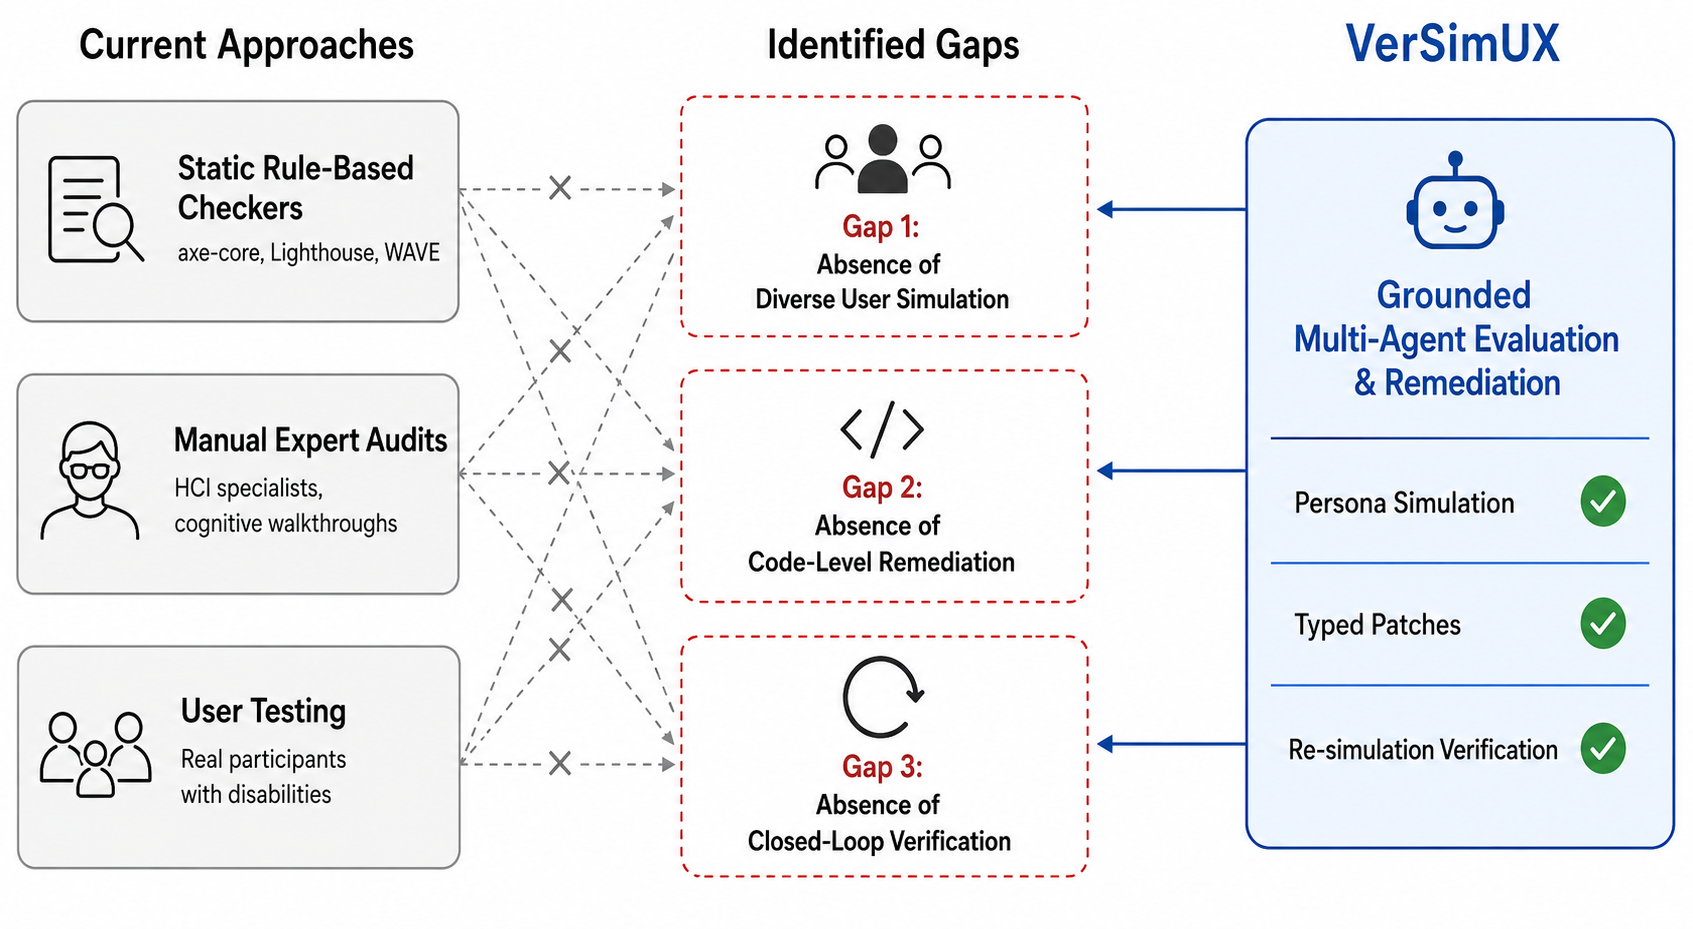
\includegraphics[width=0.92\textwidth]{static/ch01_three_gaps.png}
  \caption{The three gaps in automated web accessibility evaluation. Current approaches---static checkers, manual expert audits, and user testing---each fail to address one or more of the identified gaps. \versimux{} is designed to close all three simultaneously.}
  \label{fig:three-gaps}
\end{figure}

\subsection{Thesis Objective}

This thesis addresses all three gaps through the design, implementation, and evaluation of \versimux{}, a grounded \acrfull{MAS}{Multi-Agent System} that unifies automated diagnosis, code-level remediation, and closed-loop verification within a single orchestrated pipeline. \versimux{} operates by spawning a swarm of simulated user personas---each characterised by specific disability profiles, assistive technology configurations, technical skill levels, and behavioural tendencies---that autonomously navigate web interfaces inside real browser instances powered by Playwright. Personas execute a six-phase cognitive loop (\textit{perceive--plan--decide--execute--evaluate--reflect}) with Python-enforced grounding guards that prevent \acrfull{LLM}{Large Language Model} state hallucination, detecting usability and accessibility issues through grounded interaction rather than static analysis. A downstream pipeline of specialised agents then clusters findings using \acr{HDBSCAN} with sentence-transformer embeddings, generates typed code-level patches (HTML attributes, CSS rules, JavaScript behaviours), resolves conflicts between overlapping patches through multi-round \acr{LLM} negotiation, applies the unified patch set to the original source, and verifies the result by re-simulating failing personas on the patched interface.

The system is orchestrated as a LangGraph state graph that coordinates five specialised agent roles---supervisor, persona, recommender, conflict resolver, and verifier---across a pipeline that processes multiple pages in parallel, supports iterative correction loops, and streams real-time telemetry to a monitoring dashboard via \acrfull{SSE}{Server-Sent Events}. By grounding every evaluation in actual browser interaction and maintaining deterministic working memory in Python rather than in \acr{LLM} context, \versimux{} bridges the gap between the diagnostic capabilities of automated tools and the experiential insights of human evaluators, while producing the actionable, code-level remediation artefacts that developers need to translate findings into fixes.

\begin{figure}[ht]
  \centering
  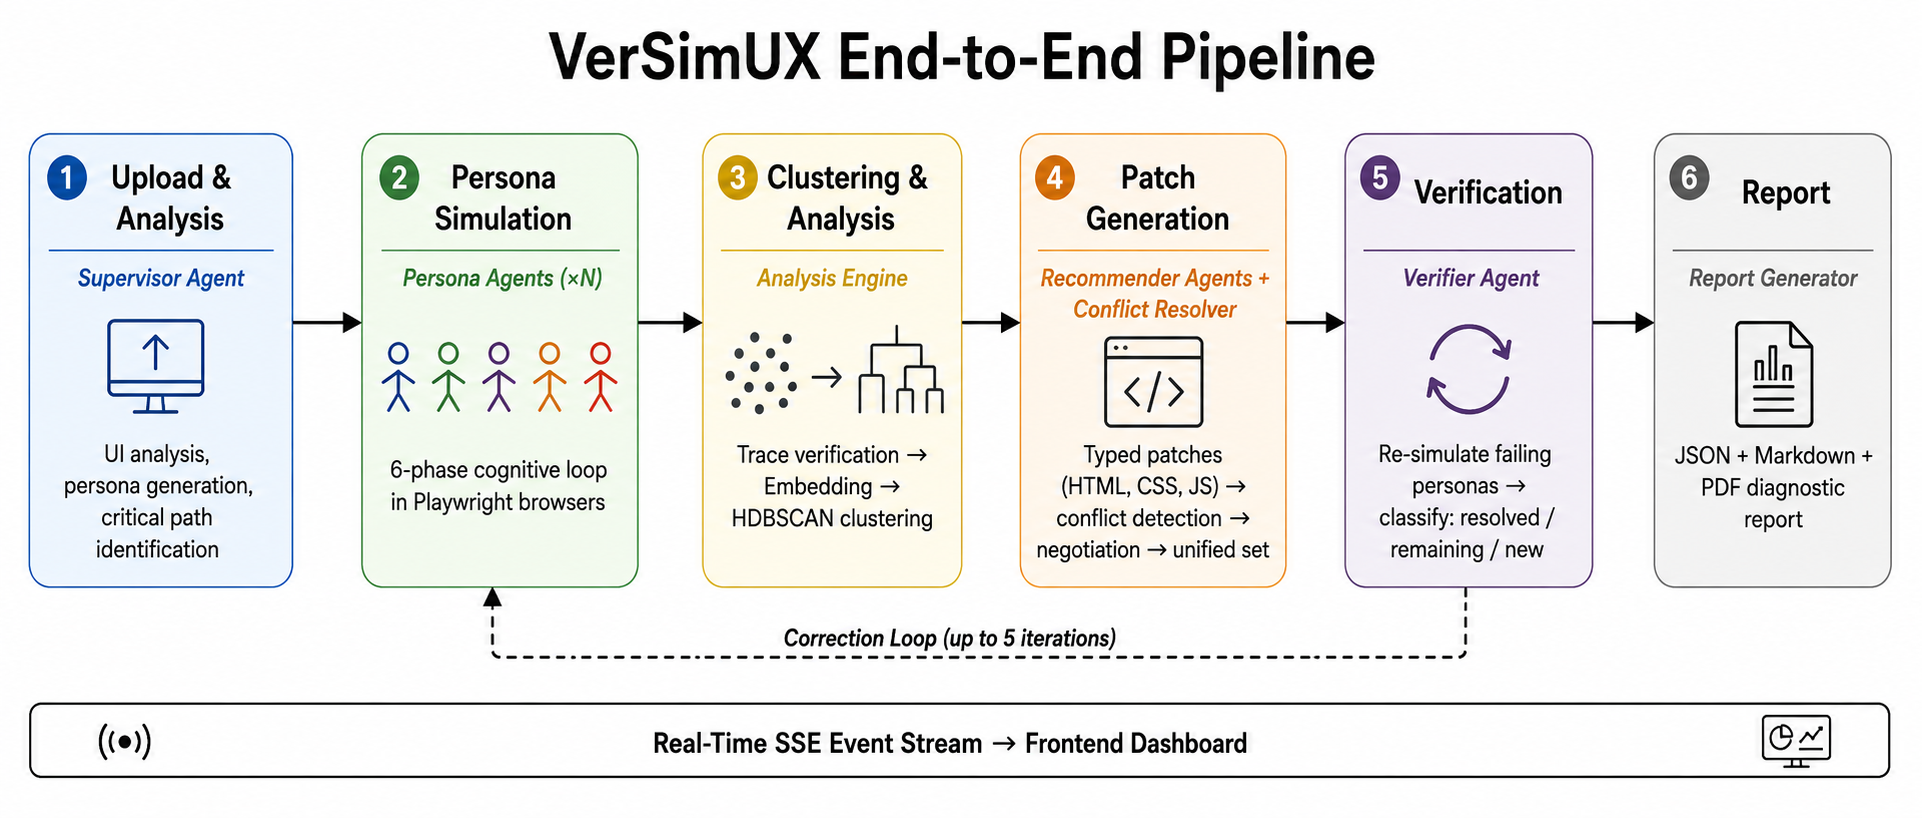
\includegraphics[width=0.95\textwidth]{static/ch01_pipeline_overview.png}
  \caption{High-level overview of the \versimux{} pipeline. HTML files are uploaded, analysed by a supervisor agent, and evaluated by a swarm of simulated personas. Findings are clustered, typed patches are generated and conflict-resolved, the unified patch set is applied, and a verification loop re-simulates failing personas to confirm effectiveness. A dashed feedback arrow indicates the iterative correction loop.}
  \label{fig:pipeline-overview}
\end{figure}


% ---- 1.2 Research Questions --------------------------------------------------
\section{Research Questions}
\label{sec:research-questions}

The three gaps identified in Section~\ref{sec:motivation} have attracted growing attention from the research community. Several recent systems have begun to explore \acr{LLM}-driven agents for interface evaluation, but each addresses only a subset of the challenges and introduces limitations that motivate the work presented in this thesis. We briefly survey five representative systems before deriving our research questions from the gaps that remain.

\subsection{Emerging Work in LLM-Based Interface Evaluation}

\paragraph{UXAgent~\cite{uxagent}.}
Xu et al. presented UXAgent at CHI~2025, an \acr{LLM} agent-based usability testing framework in which simulated users interact with live web interfaces through a browser connector. UXAgent introduces a \textit{Persona Generator Module} that synthesises diverse user profiles from researcher-defined demographic distributions, and employs dual-system reasoning---balancing fast heuristic judgements with deliberative analysis---to produce both qualitative feedback (simulated post-study surveys and think-aloud transcripts) and quantitative interaction logs. While UXAgent demonstrates that \acr{LLM} agents can approximate human-like navigation patterns and generate useful design insights, it is explicitly positioned as a \textit{study design iteration tool} rather than an end-to-end evaluation-and-remediation system. It produces unstructured diagnostic narratives but does not generate executable code patches, does not cluster or deduplicate findings across personas, and does not verify whether identified issues are resolved after intervention. Its contribution lies in demonstrating feasibility, not in closing the diagnosis-to-fix pipeline.

\paragraph{UXCascade~\cite{uxcascade}.}
Holter et al. introduced UXCascade, a scalable system that addresses the analysis bottleneck created by rapid, AI-assisted design iteration. UXCascade spins up persona-grounded \acr{LLM} agents that navigate live interfaces in parallel, records their actions and think-aloud reasoning, and---critically---aggregates unstructured agent output into a structured overview that highlights patterns across persona traits, goals, and outcomes. The system also includes an interactive fix-and-re-evaluate capability: practitioners can propose interface edits via a chat interface that generates DOM-level HTML patches, and the system automatically replays agent behaviour on the modified interface to assess impact. UXCascade thus partially addresses Gap~2 (code-level remediation) and Gap~3 (re-evaluation), but its patch generation is \textit{human-initiated}---a practitioner must manually request and review each fix through conversational interaction. The system does not autonomously generate, type, or validate patches, does not resolve conflicts between overlapping fixes, and relies on a single-shot DOM modification rather than a structured patch taxonomy. Furthermore, its re-evaluation mechanism replays the same agent trajectory rather than re-simulating under the new interface conditions, limiting its ability to detect regressions introduced by the fix.

\paragraph{ACCESS~\cite{access}.}
Huang et al. proposed ACCESS, a prompt engineering approach for automated web accessibility violation corrections. ACCESS uses the Playwright \acr{API} to systematically identify \acr{WCAG} violations, then feeds the erroneous HTML tag, error type, and violation description to a GPT model using ReAct prompting to generate corrected HTML snippets that are injected back into the \acr{DOM}. The system achieved a greater than 51\% reduction in accessibility violation errors on its benchmark dataset, demonstrating that foundation models can produce meaningful remediation code. However, ACCESS operates at the level of \textit{individual DOM elements in isolation}: it corrects one violation at a time without considering inter-patch dependencies, does not cluster related issues, and does not employ conflict resolution when multiple fixes target overlapping elements. More fundamentally, ACCESS evaluates violations through static rule-based detection (the same paradigm as axe-core), not through simulated user interaction, and therefore cannot identify the interaction-level usability issues that emerge only when diverse users navigate the interface.

\paragraph{Agentic Persona Control~\cite{agenticpersona}.}
Karthikeyan et al. presented a multi-agent framework for realistic user simulation in interactive scenarios. Their key insight is that single-\acr{LLM} user simulators lack nuance in persona adherence, exhibit excessive cooperation, and struggle with state consistency over extended interactions. To address this, they decompose the simulation into three specialised agents: a \textit{User Agent} that orchestrates the interaction flow, a \textit{State Tracking Agent} that maintains structured task state to ensure coherence, and a \textit{Message Attributes Agent} that controls conversational style based on persona and task progress. Ablation studies demonstrated significant improvements in persona adherence, task completion accuracy, and behavioural realism compared to monolithic baselines. While this work does not address web interface evaluation directly---its validation domain is restaurant ordering dialogues---it establishes an important architectural principle that \versimux{} adopts: \textit{separating cognitive concerns across specialised agents with explicit state tracking in code rather than in \acr{LLM} context} substantially improves the reliability and groundedness of persona-driven simulation.

\paragraph{AgentA/B~\cite{agentab}.}
Finally, AgentA/B automates web A/B testing by generating diverse persona-driven \acr{LLM} agents that interact with live web pages through an environment parsing module (which simplifies complex pages into structured JSON) and an action execution module (which uses browser automation to execute agent decisions). In a controlled experiment on Amazon.com involving 1,000 agents, the system demonstrated that agent behavioural trends across \acr{UI} variants were consistent with parallel human studies, though agents were more goal-directed and produced shorter action sequences. AgentA/B validates the principle that \acr{LLM} agent swarms can serve as scalable proxies for human user populations, but its focus is on comparative preference testing (which design variant performs better?) rather than diagnostic evaluation (what specific issues exist and how can they be fixed?). It does not perform accessibility evaluation, does not generate remediation patches, and does not include a verification loop.

\subsection{Remaining Gaps}

Table~\ref{tab:related-gaps} summarises the coverage of each system against the three gaps identified in Section~\ref{sec:motivation}. No existing system simultaneously addresses all three: diverse persona-driven simulation with grounded browser interaction, autonomous typed patch generation with conflict resolution, and closed-loop verification through re-simulation.

\begin{table}[ht]
\centering
\caption{Coverage of the three gaps by recent related systems.}
\label{tab:related-gaps}
\small
\renewcommand{\arraystretch}{1.2}
\begin{tabular}{@{}lccc@{}}
\toprule
\textbf{System} & \textbf{Gap 1: Simulation} & \textbf{Gap 2: Patches} & \textbf{Gap 3: Verification} \\
\midrule
UXAgent              & \checkmark & ---         & ---         \\
UXCascade            & \checkmark & Partial$^*$ & Partial$^\dagger$ \\
ACCESS               & ---         & \checkmark  & ---         \\
Agentic Persona      & \checkmark$^\ddagger$ & --- & --- \\
AgentA/B             & \checkmark & ---         & ---         \\
\midrule
\textbf{\versimux{}} & \checkmark & \checkmark  & \checkmark  \\
\bottomrule
\end{tabular}

\vspace{2mm}
\raggedright
\footnotesize
$^*$Human-initiated DOM edits, not autonomous typed patches.
$^\dagger$Trajectory replay, not re-simulation under new conditions.
$^\ddagger$Validated in dialogue, not web interface, domain.
\end{table}

\subsection{Derived Research Questions}

Building on the gaps that remain unaddressed by prior work, this thesis investigates the following research questions:

\begin{description}
  \item[RQ1 --- Diagnostic Coverage:] To what extent does \versimux{}'s persona-driven, interaction-grounded evaluation detect usability and accessibility issues that static rule-based tools (axe-core, Lighthouse) miss, and how does its diagnostic coverage compare to expert manual evaluation in terms of precision, recall, and F1 score?

  \item[RQ2 --- Grounding Effectiveness:] Do the Python-enforced working memory, action guards, and rule-based trace verification mechanisms---inspired by the cognitive decomposition principles of Karthikeyan et al.~\cite{agenticpersona}---effectively prevent hallucinated diagnoses and looping behaviours while retaining genuine usability findings?

  \item[RQ3 --- Remediation Quality:] Does \versimux{}'s autonomous patch synthesis pipeline---which generates typed code-level patches (HTML, CSS, JavaScript), detects inter-patch conflicts, and resolves them through multi-round \acr{LLM} negotiation---produce fixes that are syntactically valid, semantically correct, and applicable without introducing regressions, and how does its remediation rate compare to the single-element correction approach of ACCESS~\cite{access}?

  \item[RQ4 --- Closed-Loop Verification:] Does re-simulating failing personas on patched interfaces provide a reliable signal of remediation effectiveness, and does the iterative correction loop improve resolution rates compared to single-pass patch application as employed by UXCascade~\cite{uxcascade} and ACCESS~\cite{access}?
\end{description}


% ---- 1.3 Contributions -------------------------------------------------------
\section{Contributions}
\label{sec:contributions}

This thesis makes the following contributions, each addressing one or more of the research questions formulated in Section~\ref{sec:research-questions}:

\begin{enumerate}
  \item \textbf{A grounded persona simulation architecture (RQ1, RQ2).} We design and implement a persona agent that executes a six-phase cognitive loop---\textit{perceive, plan, decide, execute, evaluate, reflect}---inside isolated Playwright browser contexts. Each persona is characterised by a disability profile, assistive technology configuration, technical skill level, and behavioural tendency. Crucially, the agent's working memory (page phase, fields filled, steps remaining, action history) is maintained entirely in Python data structures and injected into every \acr{LLM} prompt, ensuring that the model cannot hallucinate or contradict its own state. This design directly operationalises the cognitive decomposition principle established by Karthikeyan et al.~\cite{agenticpersona} and extends it from dialogue simulation to grounded web interaction.

  \item \textbf{Deterministic action guards and trace verification (RQ2).} We introduce a suite of Python-enforced guards---scroll stagnation detection, repeat-action prevention, observe-spiral breaking, selector grounding verification, and navigation interception---that constrain persona behaviour within physically plausible interaction patterns. After simulation, a rule-based trace verifier applies heuristics (loop detection, missing selectors, network errors, unknown elements) to discard traces with greater than 40\% invalid steps before they propagate to downstream analysis. Unlike prompt-only guardrails, these mechanisms operate deterministically and cannot be circumvented by model output.

  \item \textbf{HDBSCAN-based issue clustering with semantic embeddings (RQ1).} Persona findings are deduplicated and grouped using sentence-transformer embeddings (\texttt{all-MiniLM-L6-v2}) and HDBSCAN clustering with dynamic \texttt{min\_cluster\_size}. Each cluster aggregates metadata---dominant severity, dominant category, affected personas, affected elements, and a representative description---producing a structured diagnostic output that is both machine-actionable and human-readable. This addresses a limitation shared by UXAgent~\cite{uxagent} and UXCascade~\cite{uxcascade}, neither of which clusters or deduplicates findings across multiple simulated users.

  \item \textbf{Typed, autonomous patch synthesis with conflict resolution (RQ3).} For each issue cluster, specialised recommender agents generate typed patch proposals spanning seven categories: \texttt{html\_attribute}, \texttt{html\_structure}, \texttt{content}, \texttt{css\_rule}, \texttt{css\_class}, \texttt{inline\_style}, and \texttt{js\_snippet}. When multiple patches target overlapping DOM elements, a conflict detector identifies collisions and a mediator agent resolves them through structured multi-round \acr{LLM} negotiation, producing merged or prioritised patches. This goes substantially beyond the single-element, conflict-unaware correction approach of ACCESS~\cite{access} and the human-initiated DOM editing of UXCascade~\cite{uxcascade}.

  \item \textbf{A closed-loop verification and correction mechanism (RQ4).} After patch application, a verification agent re-evaluates each original issue against the patched HTML, classifying issues as \textit{resolved}, \textit{remaining}, or \textit{new}. If the resolution rate falls below a configurable threshold (default: 80\% of critical and high-severity issues), the pipeline enters an iterative correction loop that re-simulates failing personas on the patched interface, re-clusters emerging issues, generates additional patches, and re-verifies---repeating for up to five iterations. This constitutes the first fully automated, re-simulation-based verification loop in the \acr{LLM}-driven accessibility evaluation literature.

  \item \textbf{A LangGraph-based multi-agent orchestration architecture (RQ1--RQ4).} The entire pipeline is modelled as a directed acyclic graph using LangGraph's \texttt{StateGraph}, with parallel page processing via \texttt{Send()}, type-safe state annotations with \texttt{Annotated[list, operator.add]} for concurrent write safety, and conditional edges for correction loops. This architecture coordinates five distinct agent roles---supervisor, persona, recommender, conflict resolver, and verifier---across a pipeline that scales to multiple pages and dozens of concurrent personas within a bounded thread pool.

  \item \textbf{A real-time observability and telemetry infrastructure (RQ1).} The system exposes a comprehensive event-streaming architecture based on \acr{SSE}, a thread-safe \texttt{EventBus} singleton, and a \texttt{structlog} logging bridge that automatically emits every backend log event as a structured SSE payload. Session state, events, and results are persisted to SQLite with auto-incrementing event IDs, enabling reconnection with \texttt{Last-Event-ID} tracking and full session replay after backend restarts. This infrastructure provides the observability necessary to inspect, debug, and analyse multi-agent evaluation runs in both real time and post hoc.
\end{enumerate}


% ---- 1.4 Thesis Outline ------------------------------------------------------
\section{Thesis Outline}
\label{sec:outline}

The remainder of this thesis is organised into eight chapters and four appendices, structured to move from theoretical foundations through system design to empirical validation.

\begin{description}
  \item[\Cref{ch:background} --- Background and Related Work] reviews the foundational literature across four domains: (1)~web accessibility standards and automated evaluation tools, (2)~simulated user testing and cognitive modelling, (3)~multi-agent system architectures and \acr{LLM}-based agent frameworks, and (4)~automated program repair. This chapter provides the theoretical grounding for the design decisions presented in subsequent chapters and positions \versimux{} within the existing landscape through a detailed comparison with UXAgent~\cite{uxagent}, UXCascade~\cite{uxcascade}, ACCESS~\cite{access}, and related systems.

  \item[\Cref{ch:overview} --- System Overview] provides a high-level walkthrough of the \versimux{} pipeline, from HTML upload through persona simulation, issue clustering, patch synthesis, conflict resolution, patch application, verification, and report generation. This chapter establishes the end-to-end workflow and the design principles---grounding, modularity, deterministic state management, and fail-safe degradation---that govern the architecture.

  \item[\Cref{ch:architecture} --- System Architecture] presents the detailed design and implementation of the system's core subsystems: the LangGraph pipeline topology, the supervisor agent, the persona agent with its six-phase cognitive loop and Playwright engine, the clustering engine, the recommender agent swarm, the conflict resolver, the patch applicator, the verification loop, and the report generator. Each subsystem is described in terms of its inputs, outputs, internal algorithms, and failure-handling strategies.

  \item[\Cref{ch:ai-design} --- AI and LLM Integration] discusses the \acr{LLM} integration layer in depth: prompt architecture and template design, the provider-agnostic rate limiter with per-key semaphores, the per-role \acr{LLM} router, JSON mode handling across providers, retry logic with exponential backoff, and the strategies employed to mitigate common \acr{LLM} failure modes (hallucinated selectors, malformed JSON, context window overflow, and degenerate outputs).

  \item[\Cref{ch:infrastructure} --- Runtime Infrastructure] covers the runtime environment, deployment architecture, and communication layer: the FastAPI backend with its REST and SSE endpoints, the session store with SQLite persistence and async queue broadcasting, the pipeline runner with its event mapping and heartbeat mechanism, the Playwright shared browser with thread-local caching, and the frontend dashboard architecture including the event-driven state machine and live preview system.

  \item[\Cref{ch:evaluation} --- Evaluation] presents the empirical methodology and results. This chapter describes the test corpus, evaluation metrics (precision, recall, F1 against expert baselines; patch applicability rate; regression rate; verification accuracy), experimental setup, and quantitative results for each research question. It includes ablation studies examining the contribution of individual components (grounding guards, trace verification, conflict resolution, correction loops) to overall system performance.

  \item[\Cref{ch:discussion} --- Discussion] interprets the experimental findings, analyses failure cases, discusses the limitations of \acr{LLM}-driven evaluation (model sensitivity, prompt fragility, coverage gaps for complex JavaScript-heavy interfaces), examines threats to validity, and compares \versimux{}'s performance against the related systems surveyed in \Cref{sec:research-questions}.

  \item[\Cref{ch:conclusion} --- Conclusion and Future Work] summarises the contributions of this thesis, revisits each research question with the evidence obtained, and outlines directions for future research including multi-page workflow evaluation, visual regression testing integration, fine-tuned domain-specific models, and extension to mobile native interfaces.
\end{description}

\noindent Four appendices provide supplementary material: \textbf{Appendix~A} reproduces the system configuration schema; \textbf{Appendix~B} lists the complete \acr{LLM} prompt templates; \textbf{Appendix~C} presents the Pydantic data model definitions; and \textbf{Appendix~D} provides annotated examples of full pipeline execution traces.


% ============================================================================
% Chapter 2 — Background and Related Work
% ============================================================================
\chapter{Background and Related Work}
\label{ch:background}

This chapter situates \versimux{} within the broader landscape of automated usability evaluation, simulated user testing, multi-agent systems, and automated program repair. Each section reviews the state of the art, identifies limitations that motivate the design of \versimux{}, and positions the contributions of this thesis relative to existing work.


% ---- 2.1 Automated Usability and Accessibility Evaluation --------------------
\section{Automated Usability and Accessibility Evaluation}
\label{sec:bg-accessibility}

Web accessibility evaluation, in its automated form, rests on a deceptively simple premise: that a meaningful subset of the \acr{WCAG} success criteria can be reduced to deterministic predicates over \acr{DOM} structure and computed styles. The \acr{WCAG} 2.1 standard~\cite{wcag21}, extended by version 2.2~\cite{wcag22}, organises its requirements around four principles---Perceivable, Operable, Understandable, and Robust---spanning 78 success criteria across three conformance levels (A, AA, AAA). Of these criteria, roughly 30--40\% admit fully automated verification: whether an image element carries alternative text, whether interactive controls are keyboard-reachable, whether colour contrast ratios exceed specified thresholds~\cite{abascal2004guidelines}. The remainder---criteria involving semantic clarity, cognitive load, error recovery, and consistent navigation---require human judgement that no static rule can replicate.

The most widely adopted automated checker is axe-core~\cite{axecore}, an open-source JavaScript engine developed by Deque Systems that implements over 100 \acr{WCAG} rules as \acr{DOM} traversal predicates. When injected into a browser context, axe-core queries the accessibility tree and computed style properties to produce a structured violation list containing the offending element, the violated rule identifier, and a remediation hint. Its architecture is deliberately stateless: each invocation evaluates the page as a frozen snapshot, without performing interactions or tracking state transitions. This makes axe-core fast and deterministic---properties that have driven its integration into continuous integration pipelines, browser extensions, and quality gates worldwide---but it also confines its coverage to the subset of \acr{WCAG} criteria that can be expressed as structural predicates.

Google Lighthouse~\cite{lighthouse} extends the automated auditing paradigm beyond accessibility to encompass performance, progressive web app compliance, and search engine optimisation. Its accessibility audit draws heavily on axe-core's rule set but supplements it with additional heuristics derived from Chrome's accessibility tree implementation. Lighthouse produces a numerical score (0--100) that aggregates individual rule pass rates, weighted by severity. While this scoring approach provides a convenient summary metric, Brajnik~\cite{brajnik2008comparative} demonstrated in a comparative study of evaluation methods that significant variation in the types and quantities of issues detected by each method suggests that no single automated approach---and by extension, no single aggregated score---provides a reliable picture of accessibility conformance.

Several additional tools occupy distinct niches within the automated evaluation landscape. WAVE~\cite{wave}, developed by the WebAIM initiative, overlays visual annotations directly onto the rendered page, marking violations with colour-coded icons that allow developers to inspect issues in their visual context. Pa11y~\cite{pa11y} provides a command-line interface and Node.js \acr{API} that make it straightforward to integrate accessibility checks into continuous deployment scripts, supporting multiple reporting formats and configurable rule sets. AccessLint~\cite{accesslint} takes a different architectural approach entirely, embedding itself into the GitHub pull request workflow and posting violation comments directly on the lines of code that introduce new accessibility failures. Each of these tools optimises for a different stage of the development lifecycle, yet all share the same fundamental constraint: they evaluate code, not user experience.

The limitations of static rule checking have been recognised since the earliest efforts to automate accessibility verification. Abascal et al.~\cite{abascal2004guidelines} showed that guideline-based checkers achieve high precision for structural rules but produce both false positives---flagging technically non-compliant patterns that are functionally accessible---and false negatives---missing violations that depend on interaction context. More recently, the WebAIM Million report~\cite{webaim_million}, which annually evaluates the home pages of the top one million websites, has consistently found that pages scoring well on automated checks still exhibit pervasive usability barriers when assessed by users with disabilities. The implication is clear: automated accessibility evaluation as currently practised addresses only the most tractable portion of the problem, leaving the interaction-dependent, context-sensitive, and user-subjective dimensions of usability and accessibility largely unexamined.

\begin{table}[htbp]
  \centering
  \caption{Comparison of existing automated accessibility evaluation tools.}
  \label{tab:tool-comparison}
  \begin{tabularx}{\textwidth}{@{}l L{2.5cm} L{2.5cm} C{1.8cm} C{1.8cm} C{1.8cm}@{}}
    \toprule
    \textbf{Tool} & \textbf{Method} & \textbf{Output Type} & \textbf{Multi-User Sim.} & \textbf{Code Patches} & \textbf{Verification} \\
    \midrule
    axe-core        & Static rule checking      & Violation list       & No  & No  & No  \\
    Lighthouse      & Static + performance      & Audit report         & No  & No  & No  \\
    WAVE            & Visual overlay            & Annotated page       & No  & No  & No  \\
    Pa11y           & Automated rule runner     & Violation list       & No  & No  & No  \\
    AccessLint      & CI/CD integration         & PR comments          & No  & No  & No  \\
    \midrule
    \versimux{}     & Simulated persona agents  & Patches + report     & Yes & Yes & Yes \\
    \bottomrule
  \end{tabularx}
\end{table}

\Cref{tab:tool-comparison} summarises the capabilities and limitations of the tools surveyed in this section. The final row positions \versimux{}, which addresses the three missing capabilities---multi-user simulation, code-level patches, and automated verification---through the agent-based architecture described in \cref{ch:overview,ch:architecture}.


% ---- 2.2 Simulated Users and Agentic Usability Testing ----------------------
\section{Simulated Users and Agentic Usability Testing}
\label{sec:bg-simulated-users}

The idea of modelling user behaviour computationally predates the web itself. The \acrfull{GOMS}{Goals, Operators, Methods, and Selection rules} family of models, systematised by John and Kieras~\cite{john1996goms}, decomposes task execution into a hierarchy of goals, cognitive and motor operators (e.g., perceiving a label, pressing a key), methods for achieving goals, and selection rules for choosing among alternative methods. The simplest member of the family, the \acrfull{KLM}{Keystroke-Level Model}, predicts task completion time by summing operator durations along a predetermined action sequence. \acr{GOMS} models are deterministic, analytically tractable, and have demonstrated strong predictive validity for routine, well-practised tasks~\cite{john1996goms}. They remain a standard reference point in \acr{HCI} curricula and usability engineering practice.

John et al.~\cite{cogtool} operationalised \acr{GOMS} prediction through CogTool, a prototyping tool that allows interface designers to define storyboard-style task sequences and automatically derive \acr{KLM}-level timing predictions from the specified interactions. CogTool made cognitive modelling accessible to practitioners who lacked formal training in cognitive psychology, demonstrating that useful performance predictions could be obtained from lightweight interface mockups rather than full implementations. However, \acr{GOMS}-based approaches share two structural limitations that constrain their applicability to accessibility evaluation. First, they require the analyst to predefine the complete action sequence---they cannot generate novel interaction paths or respond to unexpected interface states. Second, they model a single, idealised user profile and cannot represent the diversity of abilities, strategies, and assistive technology configurations that characterise real user populations.

The emergence of \acr{LLM}-based autonomous agents has fundamentally altered the landscape of simulated user testing. Rather than following predefined action sequences, \acr{LLM} agents observe the current interface state, reason about their goals, and select actions through natural language understanding of the \acr{DOM}. This capability has motivated the development of realistic evaluation environments. WebArena~\cite{zhou2024webarena} provides a self-hosted web environment comprising four fully functional web applications---e-commerce, forums, code management, and content management---that serve as standardised benchmarks for measuring agent task completion rates. Mind2Web~\cite{deng2023mind2web} complements this with a large-scale dataset of over 2,000 open-ended web tasks across 137 real-world websites, annotating the ground-truth action sequences that human users follow. Together, these resources have established the empirical foundation for evaluating whether \acr{LLM} agents can navigate complex web interfaces with sufficient fidelity to serve as proxies for human users.

Building on these foundations, several research groups have explored \acr{LLM} agents specifically for usability and design evaluation. As surveyed in \cref{sec:research-questions}, UXAgent~\cite{uxagent} demonstrated that persona-grounded agents can generate qualitative feedback that approximates the outputs of human testers, UXCascade~\cite{uxcascade} introduced scalable parallel evaluation with an interactive fix-and-retest workflow, and AgentA/B~\cite{agentab} validated the principle that agent swarms can approximate human behavioural distributions in A/B testing scenarios. These systems collectively establish that \acr{LLM}-based agents represent a viable paradigm for simulated user testing at scale.

Despite these advances, a fundamental tension pervades the paradigm. The same flexibility that enables \acr{LLM} agents to generate diverse, creative interaction sequences also allows them to produce traces that are plausible but not grounded in the actual interface state. An agent may report clicking a button that does not exist in the rendered page, describe a visual layout that differs from the computed styles, or hallucinate accessibility violations based on patterns memorised during pre-training rather than on evidence observed in the current session. Without explicit mechanisms to anchor agent perception and action in the live \acr{DOM}, the diagnostic outputs of \acr{LLM}-based evaluators remain fundamentally unverifiable---a challenge that motivates the grounding architecture discussed in \cref{sec:bg-grounding}.


% ---- 2.3 Multi-Agent Systems for Software Engineering -----------------------
\section{Multi-Agent Systems for Software Engineering}
\label{sec:bg-mas}

A multi-agent system (\acr{MAS}) consists of multiple autonomous entities---\textit{agents}---that perceive their environment, maintain internal state, act upon the environment, and coordinate with one another to achieve individual or collective objectives~\cite{wooldridge2009mas}. Wooldridge identifies four properties that distinguish agents from ordinary software components: \textit{autonomy} (operating without direct external control), \textit{reactivity} (responding to environmental changes), \textit{proactivity} (taking initiative to satisfy goals), and \textit{social ability} (interacting with other agents through defined protocols). These properties make multi-agent architectures particularly suited to problems that require diverse expertise, parallel execution, and decentralised decision-making---all characteristics of comprehensive usability evaluation.

The dominant theoretical framework for deliberative agent design is the \acrfull{BDI}{Belief-Desire-Intention} architecture, introduced by Rao and Georgeff~\cite{rao1995bdi}. In a \acr{BDI} agent, \textit{beliefs} represent the agent's current knowledge of its environment, \textit{desires} encode the goals it seeks to achieve, and \textit{intentions} constitute the committed plans it is currently executing. The deliberation cycle continuously updates beliefs from environmental perception, selects desires that are consistent with current beliefs, and commits to intention plans that advance the selected desires. This framework provides a principled basis for reasoning about agent behaviour: an agent's actions can be explained and predicted through the logical relationships among its beliefs, desires, and intentions. \versimux{}'s persona agents embody a simplified variant of the \acr{BDI} cycle: beliefs are grounded in the \acr{DOM} state extracted by the Playwright engine, desires are derived from persona task goals assigned by the supervisor, and intentions are constrained by Python-enforced action guards that prevent the agent from committing to infeasible plans.

Park et al.~\cite{park2023generative} demonstrated that \acr{LLM}-powered agents can exhibit surprisingly believable human behaviour when equipped with appropriate memory and reflection mechanisms. Their \textit{Generative Agents} architecture endows each agent with a memory stream (a time-stamped record of observations and actions), a retrieval mechanism that surfaces contextually relevant memories, and a reflection process that synthesises higher-level insights from accumulated experience. In a simulated town environment, 25 such agents formed social relationships, coordinated group activities, and exhibited emergent behaviours that human evaluators judged more believable than hand-scripted character responses. This work established the empirical viability of \acr{LLM}-based agent simulation at scale and introduced the architectural pattern of separating memory, retrieval, and reflection into distinct computational modules---a pattern that \versimux{} adapts through its WorkingMemory dataclass and its decomposition of persona cognition into a six-phase pipeline of perception, planning, decision, execution, evaluation, and reflection.

The application of \acr{MAS} architectures to software engineering tasks has yielded particularly relevant precedents. MetaGPT~\cite{metagpt} introduced a multi-agent framework in which \acr{LLM} agents are assigned distinct software engineering roles---product manager, architect, engineer, tester---and collaborate through structured message passing with standardised output artefacts (requirements documents, design diagrams, code files, test reports). By encoding human workflow conventions into the agent coordination protocol, MetaGPT demonstrated that role specialisation with structured inter-agent communication substantially reduces cascading hallucination errors compared to monolithic, single-agent approaches. SWE-agent~\cite{sweagent} complemented this finding by showing that the design of the agent--computer interface itself critically affects agent performance: providing agents with purpose-built tools for navigating codebases, editing files, and running tests improved issue resolution rates on the SWE-bench benchmark far more than simply upgrading the underlying \acr{LLM}. Both findings directly inform \versimux{}'s architecture, which assigns five specialised roles (supervisor, persona, recommender, conflict resolver, and verifier) and provides each role with domain-specific tooling (browser engine, \acr{DOM} state extractor, patch applicator) rather than relying on generic \acr{LLM} prompting alone.

The orchestration of multi-agent workflows in \versimux{} relies on LangGraph~\cite{langgraph}, a framework that models agent pipelines as directed state graphs with typed state containers. Unlike simple sequential chains or reactive event loops, LangGraph's state graph model supports three capabilities that prove essential for the \versimux{} pipeline: (1)~\textit{parallel fan-out} via the \code{Send()} primitive, enabling multiple pages and personas to be processed concurrently; (2)~\textit{conditional edges} that implement branching logic such as the correction loop triggered by failed verification; and (3)~\textit{typed state annotations} using Python's \code{Annotated} type hints, which ensure that concurrent node writes to shared state (e.g., appending results from parallel branches to a shared list) are handled safely without explicit locking. This combination of parallelism, conditionality, and type safety distinguishes LangGraph from earlier \acr{MAS} coordination mechanisms that relied on message queues, blackboard architectures, or ad hoc scripting.


% ---- 2.4 LLM Grounding, Hallucination, and Trust ---------------------------
\section{LLM Grounding, Hallucination, and Trust}
\label{sec:bg-grounding}

\acr{LLM} hallucination---the generation of content that is fluent and confident but factually incorrect or inconsistent with the provided input---represents the central reliability challenge for agentic systems operating in interactive environments. Ji et al.~\cite{ji2023hallucination} provide a comprehensive taxonomy distinguishing \textit{intrinsic} hallucinations (outputs that contradict the source material) from \textit{extrinsic} hallucinations (outputs that introduce claims neither supported nor contradicted by the source). In the context of web agent systems, hallucination manifests in particularly damaging forms: agents may reference \acr{DOM} elements that do not exist, describe visual properties that differ from the computed styles, report interaction outcomes that never occurred, or fabricate accessibility violations based on patterns memorised during pre-training rather than on evidence observed in the current page. When the purpose of the agent is to produce a diagnostic evaluation, hallucinated findings are indistinguishable from genuine ones without an independent verification mechanism.

The ReAct framework~\cite{yao2023react} addressed a closely related challenge---the disconnect between reasoning and action in language models---by proposing an interleaved thought--action--observation loop. In ReAct, the model alternates between generating free-form reasoning traces (``I need to find the search bar''), executing concrete actions (``click element \#search-input''), and incorporating observations from the environment (``the page now shows a text input with placeholder `Search\ldots'\,''). This interleaving forces the model to ground each reasoning step in an observed environmental state, reducing the accumulation of unsupported inferences that occurs in pure chain-of-thought reasoning. \versimux{}'s persona agent adopts a similar interleaved structure---the six-phase cognitive pipeline alternates between perception (\acr{DOM} state extraction), reasoning (plan and decision phases), action (Playwright execution), and evaluation (outcome assessment)---but extends it with deterministic, Python-enforced constraints that ReAct's prompt-only approach cannot guarantee.

A complementary grounding strategy, explored by Schick et al.~\cite{schick2023toolformer} in Toolformer, teaches language models to recognise when their own parametric knowledge is insufficient and to delegate specific subtasks to external tools---calculators, search engines, translation services---rather than attempting to generate answers from memory alone. The central insight is that tool use provides a \textit{verifiable} grounding mechanism: the output of a calculator can be checked, the result of a search query can be traced to a source document, and the return value of an \acr{API} call can be validated against a schema. In web agent systems, this principle translates to the use of browser automation \acr{API}s as grounding instruments: rather than asking the \acr{LLM} to describe what it ``sees'' on a page, the system extracts the \acr{DOM} state programmatically and presents it to the model as a structured observation that reflects the actual page content.

The benchmarks established by WebArena~\cite{zhou2024webarena} and Mind2Web~\cite{deng2023mind2web} have quantified the severity of the grounding problem in practice. On WebArena's task suite, even the strongest \acr{LLM} agents achieve task completion rates well below 20\%, with failure analysis revealing that a substantial fraction of errors stem from hallucinated selectors, incorrect assumptions about page state, and actions that target elements not interactable in the current \acr{DOM} configuration. These findings underscore that raw \acr{LLM} capability---even with frontier models---is insufficient for reliable web interaction without additional mechanisms to verify the feasibility and correctness of proposed actions before they are executed.

An instructive parallel exists in robotics. Ahn et al.~\cite{saycan} introduced SayCan, a system that grounds language model plans in robotic affordances: before executing a natural-language instruction (``bring me a sponge from the kitchen counter''), the system queries a learned affordance function that estimates whether each candidate action is physically feasible given the robot's current state and capabilities. Actions that the language model proposes but that the robot cannot physically execute are filtered out before they reach the motor system. This \textit{affordance grounding} pattern---using an environmental feasibility check to gate \acr{LLM} output before execution---directly informs \versimux{}'s grounding architecture. In \versimux{}, the affordance function takes the form of a \acr{DOM} selector existence check: before executing any click, type, or hover action, the Playwright engine verifies that the target selector exists in the live page and is interactable, preventing hallucinated interactions from corrupting the simulation trace.

Beyond selector verification, \versimux{} implements a multi-layered grounding architecture that includes Python-maintained working memory (ensuring the \acr{LLM} cannot contradict or fabricate its own state), five deterministic action guards (preventing degenerate interaction patterns such as infinite scrolling, repeated clicking, and observation spirals), and a post-simulation trace verifier that discards traces with excessive invalid steps before they propagate to downstream analysis. The design rationale and implementation details of these mechanisms are presented in \cref{ch:architecture,ch:ai-design}.


% ---- 2.5 Automated Program Repair and Patch Synthesis -----------------------
\section{Automated Program Repair and Patch Synthesis}
\label{sec:bg-apr}

\acrfull{APR}{Automated Program Repair} is the field concerned with automatically generating source-code modifications---patches---that correct software defects. The dominant paradigm, known as \textit{generate-and-validate}, proceeds in two phases: a generation phase that proposes candidate patches through various strategies (mutation, search, semantic analysis, or machine learning), and a validation phase that evaluates each candidate against a test suite or specification to determine whether it resolves the defect without introducing regressions~\cite{legoues2012genprog}.

Le Goues et al.~\cite{legoues2012genprog} established the field with GenProg, a search-based repair technique that applies genetic programming to the abstract syntax tree of buggy programs. GenProg defines mutation operators---insert, delete, and replace---that draw repair material from elsewhere in the same program, operating under the assumption that correct code for fixing a defect often already exists in the codebase, merely in the wrong location. Candidate patches are evaluated against a test suite, and a fitness function guides the evolutionary search towards patches that pass failing tests without breaking passing ones. While GenProg demonstrated that non-trivial bugs in large C programs could be repaired automatically, subsequent analysis revealed that a significant proportion of its patches were \textit{overfitting}: they passed the test suite by deleting functionality or suppressing error paths rather than by genuinely correcting the underlying defect.

Nguyen et al.~\cite{nguyen2013semfix} addressed the overfitting problem through SemFix, a semantic repair approach that uses symbolic execution and constraint solving to synthesise patches that are correct by construction with respect to a formal specification of the expected behaviour. By reasoning about program semantics rather than manipulating syntax, SemFix produces patches that are more likely to generalise beyond the specific test inputs used for validation. However, the computational cost of symbolic execution limits the approach to relatively small programs and localised defects, making it impractical for the scale and diversity of modifications that accessibility remediation typically requires.

The advent of \acr{LLM}s has introduced a third paradigm for program repair. Xia and Zhang~\cite{xia2023apr} conducted a systematic study of \acr{LLM}-based \acr{APR}, demonstrating that pre-trained code models can generate correct patches by treating repair as a conditional generation task: given the buggy code, the test failure message, and optionally the surrounding context, the model generates a modified code fragment. Their results showed that \acr{LLM}-based approaches substantially outperformed both search-based and semantic methods on established benchmarks, benefiting from the models' capacity to learn repair patterns from the vast corpus of code changes observed during pre-training. However, the authors noted that \acr{LLM}-generated patches are susceptible to the same hallucination risks identified in \cref{sec:bg-grounding}: models may generate syntactically plausible but semantically incorrect fixes, particularly when the repair requires domain-specific knowledge not well represented in the training data.

The application of \acr{APR} to \acr{UI} accessibility repair introduces domain-specific challenges that none of the techniques reviewed above directly address. First, \acr{UI} repairs span three distinct languages (HTML, CSS, and JavaScript), each with different semantics and failure modes---a single remediation effort that adds an \code{aria-label} attribute (HTML), adjusts a contrast ratio (CSS), and installs a keyboard event handler (JavaScript) requires coordinated modifications across all three languages for a single element. Second, \acr{UI} patches interact visually and behaviourally: two patches targeting the same element may produce conflicting styles, overlapping event handlers, or redundant \acr{ARIA} attributes. Standard \acr{APR} techniques, which validate patches against functional test suites, cannot evaluate these visual and interactive side effects. Third, the ``test suite'' for accessibility repair is not a set of unit tests but the subjective experience of users with diverse abilities---a criterion that resists straightforward programmatic specification. As discussed in \cref{sec:research-questions}, ACCESS~\cite{access} represents a notable step towards \acr{LLM}-based accessibility repair, but it operates on individual elements in isolation without conflict awareness or verification. \versimux{} addresses these challenges through a typed patch taxonomy spanning seven categories, an explicit conflict detection and resolution protocol, and a verification mechanism that re-simulates user personas on the patched interface rather than relying on traditional test suites.


% ---- 2.6 Developer-Facing Accessibility Tooling -----------------------------
\section{Developer-Facing Accessibility Tooling}
\label{sec:bg-dev-tools}

Beyond the research tools surveyed in the preceding sections, a substantial ecosystem of developer-facing accessibility tooling has emerged, designed to integrate accessibility evaluation into the daily workflows of frontend engineers. These tools vary in their integration points---browser extensions, linting rules, continuous integration hooks, code review bots---but share a common output paradigm: they identify violations and provide textual guidance on how to fix them, without generating executable code changes.

The most comprehensive commercial ecosystem is maintained by Deque Systems, the developers of axe-core~\cite{axecore}. Deque's product suite includes axe DevTools (a browser extension that provides in-context violation highlighting and guided remediation flows), axe Monitor (a continuous scanning service that tracks accessibility compliance across entire web properties over time), and axe Auditor (a workflow management platform for professional audit teams). While these tools significantly reduce the effort required to \textit{identify} accessibility issues, their remediation guidance takes the form of textual suggestions---``add an \code{alt} attribute to this image'', ``ensure this form input has a visible label''---that the developer must manually interpret and implement in code.

A parallel category of tools embeds accessibility checks directly into the software development lifecycle. AccessLint~\cite{accesslint} analyses pull requests on GitHub and posts violation comments on the specific lines of code that introduce new accessibility failures, enabling developers to address regressions before they reach production. Pa11y~\cite{pa11y} provides a command-line interface that can be integrated into continuous deployment pipelines, failing builds that exceed configurable violation thresholds. Linting plugins such as \code{eslint-plugin-jsx-a11y} check component code for common accessibility anti-patterns during development, providing immediate feedback in the editor. These integrations shift accessibility evaluation \textit{left} in the development process---closer to the point of code creation---but do not fundamentally alter the output format: the developer still receives a violation report and must independently craft the fix.

The persistent gap across the entire developer tooling landscape is the absence of \textit{actionable remediation artefacts}---concrete, executable code changes that developers can review, test, and apply rather than interpret and rewrite from scratch. This gap is not merely a convenience issue; it represents a meaningful barrier to accessibility adoption in practice. The cognitive effort required to translate a diagnostic finding (``WCAG 1.3.1: Form input missing programmatic label'') into a working fix (adding an \code{aria-label} attribute, wrapping the input in a \code{<label>} element, or restructuring the form with \code{<fieldset>} and \code{<legend>}) demands accessibility expertise that many development teams lack. By generating typed, conflict-resolved, and verified code patches, \versimux{} aims to reduce this translation burden from a specialised skill requirement to a code review task that any frontend developer can evaluate.


% ---- 2.7 Summary and Research Gap -------------------------------------------
\section{Summary and Research Gap}
\label{sec:bg-gap}

The preceding sections have surveyed six domains that collectively provide the intellectual and technical foundations for \versimux{}: automated accessibility evaluation (\cref{sec:bg-accessibility}), simulated user testing (\cref{sec:bg-simulated-users}), multi-agent system architectures (\cref{sec:bg-mas}), \acr{LLM} grounding (\cref{sec:bg-grounding}), automated program repair (\cref{sec:bg-apr}), and developer-facing tooling (\cref{sec:bg-dev-tools}). Each domain contributes essential capabilities---diagnostic rule engines, cognitive user models, agent coordination protocols, grounding mechanisms, patch generation strategies, and workflow integration patterns---but none provides a complete solution to the three gaps identified in \cref{sec:motivation}.

Static checkers and developer tools can evaluate code structure but cannot simulate user experience. Cognitive models and \acr{LLM} agents can simulate user behaviour, but without grounding they cannot guarantee that their observations correspond to reality. \acr{MAS} frameworks provide the coordination infrastructure for parallel evaluation and remediation, but they are inherently domain-agnostic and require task-specific agent designs and tools. \acr{APR} techniques can generate code patches, but they have not been adapted to the multi-language, visually interactive, conflict-prone domain of \acr{UI} accessibility. Grounding mechanisms can anchor agent actions in environmental state, but they have not been integrated into usability evaluation systems in a way that preserves both diagnostic flexibility and interaction reliability.

\begin{figure}[htbp]
  \centering
  \framebox[\textwidth]{\rule{0pt}{7.5cm}\parbox{0.9\textwidth}{\centering\large\sffamily [Figure 2.1: Related Work Domains Taxonomy vs. Research Gaps]\\ \vspace{1.2em} \normalsize\normalfont Displays the taxonomy of the six related literature domains evaluated in this chapter (Usability Testing, Accessibility Checkers, Multi-Agent Systems, Grounded AI, Program Repair, and Developer Tooling). The diagram maps each domain against the three research gaps, highlighting how \versimux{} synthesises these capabilities to close all three gaps simultaneously.}}
  \caption{Mapping of related research domains to the three identified usability and accessibility automation gaps.}
  \label{fig:bg-gaps-mapping}
\end{figure}

No existing body of work---whether a single tool, a research system, or a combination of techniques from the domains reviewed---simultaneously provides (1)~diverse, grounded persona simulation through real browser interaction, (2)~autonomous generation of typed, conflict-aware code patches across HTML, CSS, and JavaScript, and (3)~closed-loop verification through re-simulation of failing personas on the patched interface. This three-fold gap constitutes the research opportunity that \versimux{} addresses. The remainder of this thesis describes the architecture (\cref{ch:overview,ch:architecture}), \acr{LLM} integration design (\cref{ch:ai-design}), and runtime infrastructure (\cref{ch:infrastructure}) of the system, followed by an empirical evaluation (\cref{ch:evaluation}) that assesses the extent to which \versimux{} closes each gap.


% ============================================================================
% Chapter 3 — System Overview
% ============================================================================
\chapter{System Overview}
\label{ch:overview}

This chapter provides a high-level walkthrough of the \versimux{} system before the detailed architectural exposition in \cref{ch:architecture}. It introduces the design goals, presents the end-to-end pipeline, describes the technology stack, and discusses key architectural trade-offs.


% ---- 3.1 Design Goals and Principles ----------------------------------------
\section{Design Goals and Principles}
\label{sec:design-goals}

The design of \versimux{} is guided by five principles:

\begin{description}
  \item[Grounding.] Every agent action must be validated against the live \acrfull{DOM}{Document Object Model} before execution. Selectors that do not exist in the current page state are rejected, preventing hallucinated interactions.

  \item[Closed-Loop Remediation.] The system does not terminate at diagnosis. It synthesises concrete, typed code patches (HTML, CSS, JavaScript), applies them, and verifies their effectiveness---re-entering the evaluation loop if the resolution threshold is not met.

  \item[Actionability.] Output artifacts must be directly usable by developers: code patches that can be applied to source files, not textual suggestions that require manual interpretation.

  \item[Observability.] Every pipeline stage emits structured events that are persisted, streamed to the frontend in real time, and available for post-hoc analysis.

  \item[Provider Agnosticism.] The \acr{LLM} integration layer abstracts over multiple providers (Groq, OpenAI, DeepSeek, Qwen, Moonshot), enabling model substitution without architectural changes.
\end{description}


% ---- 3.2 End-to-End Pipeline Walkthrough ------------------------------------
\section{End-to-End Pipeline Walkthrough}
\label{sec:pipeline-walkthrough}

\begin{figure}[htbp]
  \centering
  \framebox[\textwidth]{\rule{0pt}{7cm}\parbox{0.9\textwidth}{\centering\large\sffamily [Figure 3.1: Full System Architecture Diagram]\\ \vspace{1em} \normalsize\normalfont Displays the three-tier design of \versimux{}: the Next.js Nexus client, the FastAPI backend API server with SQLite and the event bus, and the core LangGraph multi-agent pipeline.}}
  \caption{Overall system architecture showing the three-tier design: frontend client, backend API server, and the LangGraph agent pipeline.}
  \label{fig:system-architecture}
\end{figure}

The \versimux{} pipeline processes a single HTML document through twelve sequential stages:

\begin{enumerate}
  \item \textbf{HTML Upload.} The user submits an HTML file and an optional UI context description via the REST \acrfull{API}{Application Programming Interface}.

  \item \textbf{Supervisor Analysis.} The supervisor agent analyses the HTML structure, identifies interactive elements, critical user paths, and accessibility risk indicators.

  \item \textbf{Persona Generation.} Based on the analysis, the supervisor generates a diverse set of persona profiles with distinct accessibility constraints, cognitive characteristics, and task goals.

  \item \textbf{Persona Simulation.} Each persona agent executes its task goal inside an isolated Playwright browser context, producing an interaction trace with screenshots and inline issue annotations.

  \item \textbf{Trace Verification.} Rule-based heuristics validate each trace for structural integrity: loop detection, selector existence, navigate interception, and action validity.

  \item \textbf{Issue Extraction.} Verified issues from all personas are aggregated into a unified issue set.

  \item \textbf{Issue Clustering.} Sentence-transformer embeddings and HDBSCAN clustering group semantically similar issues, eliminating cross-persona duplicates.

  \item \textbf{Recommender Profile Generation.} The supervisor creates a \code{RecommenderProfile} for each cluster, specifying the fix focus, strategy hint, and priority.

  \item \textbf{Patch Synthesis.} Parallel recommender agents propose typed patches for their assigned clusters.

  \item \textbf{Conflict Resolution.} A conflict resolver detects overlapping patches and resolves them through LLM-mediated negotiation or heuristic tiebreaking.

  \item \textbf{Patch Application \& Verification.} Patches are applied to the HTML in dependency order. A verification agent assesses whether targeted issues have been resolved. If the resolution threshold is not met, the pipeline enters a correction loop.

  \item \textbf{Report Generation.} A comprehensive diagnostic report is generated with scores, issue details, applied patches, and verification results.
\end{enumerate}

\begin{figure}[htbp]
  \centering
  \framebox[\textwidth]{\rule{0pt}{7cm}\parbox{0.9\textwidth}{\centering\large\sffamily [Figure 3.2: Pipeline Stage Sequence Diagram]\\ \vspace{1em} \normalsize\normalfont Illustrates the temporal progression and state changes across the twelve pipeline stages, highlighting the iterative correction loop between patch verification and persona re-simulation.}}
  \caption{The twelve-stage pipeline sequence from HTML upload to report generation.}
  \label{fig:pipeline-sequence}
\end{figure}


% ---- 3.3 Technology Stack ----------------------------------------------------
\section{Technology Stack}
\label{sec:tech-stack}

\Cref{tab:tech-stack} summarises the key technologies employed at each architectural layer.

\begin{table}[htbp]
  \centering
  \caption{Technology stack by architectural layer.}
  \label{tab:tech-stack}
  \begin{tabularx}{\textwidth}{@{}l L{3cm} X@{}}
    \toprule
    \textbf{Layer} & \textbf{Technology} & \textbf{Purpose} \\
    \midrule
    Orchestration      & LangGraph            & State-graph pipeline with typed state, conditional edges, and parallel fan-out via \code{Send()} \\
    \acr{LLM} Backend  & Groq, OpenAI, etc.   & Provider-agnostic \acr{LLM} calls with per-role model routing and rate limiting \\
    Browser Automation & Playwright (Chromium) & Headless browser control with isolated contexts per persona \\
    Embeddings         & sentence-transformers & Issue text embedding for semantic clustering \\
    Clustering         & HDBSCAN              & Density-based clustering with automatic cluster count \\
    Backend \acr{API}  & FastAPI              & REST endpoints and \acr{SSE} streaming \\
    Persistence        & SQLite               & Session and event storage \\
    Frontend           & Next.js (React)      & Dashboard, upload interface, and report viewer \\
    \bottomrule
  \end{tabularx}
\end{table}


% ---- 3.4 Architectural Constraints and Trade-offs ----------------------------
\section{Architectural Constraints and Trade-offs}
\label{sec:trade-offs}

Several architectural decisions reflect deliberate trade-offs:

\paragraph{LangGraph over linear orchestration.}
Linear orchestration scripts are inherently brittle when applied to complex agentic workflows that require branching, error recovery, or feedback loops. A simple sequential execution path cannot easily accommodate the loopback flows required for closed-loop remediation, where failing verification results trigger a return to persona simulation. By using LangGraph, \versimux{} models the evaluation and remediation pipeline as a directed state graph. This formal structure supports conditional edges to route execution back to earlier phases, parallel fan-out via the \code{Send()} primitive to evaluate multiple HTML documents and personas concurrently, and typed state accumulation. Crucially, LangGraph's state design allows parallel branches to merge their results into a unified, type-safe schema using custom reducer functions (e.g., \code{operator.add}), eliminating the need to write custom concurrency locks or synchronization primitives.

\paragraph{ThreadPoolExecutor over asyncio for persona simulation.}
While asynchronous I/O via Python's \code{asyncio} is highly efficient for network-bound operations, integrating it with browser automation libraries like Playwright introduces significant event-loop complexity when scaled across multiple concurrent instances. Parallel browser automation runs frequently block the event loop, causing timeouts and race conditions in LLM prompt generation and DOM interaction. Furthermore, if a single page simulation crashes or hangs, isolating the event loop failure can be challenging. \versimux{} resolves these reliability concerns by using sync-mode Playwright wrapped in OS-level threads managed by a \code{ThreadPoolExecutor}. This model provides robust thread-local isolation: each persona agent maintains its own thread, its own Chromium browser context, and independent error boundaries. The slightly higher memory overhead of system threads is a worthwhile trade-off for the increased stability and cleaner exception handling during concurrent simulations.

\paragraph{SQLite over Redis for event persistence.}
To support real-time user-interface telemetry and SSE streaming, the backend requires a persistent database to record job events, telemetry logs, and diagnostic states. While dedicated in-memory stores like Redis are standard for high-throughput streaming architectures, they introduce external system daemon dependencies, increasing the complexity of setup and local deployment. Because \versimux{} is designed as a developer-facing tool running locally or in single-host container environments, high-throughput clustering is unnecessary. A local SQLite database configured with Write-Ahead Logging (WAL) and synchronous mode set to normal offers sufficient write performance (exceeding hundreds of transactions per second) and concurrent read safety, while maintaining a single-file, zero-dependency deployment model.

\paragraph{Python-maintained working memory over LLM self-tracking.}
In multi-turn web navigation simulations, the persona agent must track its operational state (e.g., active page context, target form fields filled, remaining interaction steps, and past action history). Allowing the underlying \acr{LLM} to self-track this state through prompt instructions or conversational memory inevitably leads to cognitive drift, where the model forgets its remaining step budget, hallucinates having filled non-existent inputs, or enters repetitive interaction loops. \versimux{} avoids this failure mode by keeping the agent's core working memory strictly in Python data structures (specifically, the \code{WorkingMemory} dataclass). After each browser interaction, the Python runtime updates the state variables, counts down the step budget, and formats this structured state to be injected into the next LLM prompt. This hybrid approach ensures that the model remains grounded in physical reality, preventing context hallucination while leveraging the LLM's reasoning power for action decision-making.

% ============================================================================
% Chapter 4 — System Architecture and Implementation
% ============================================================================
\chapter{System Architecture and Implementation}
\label{ch:architecture}

This chapter presents the detailed design and implementation of \versimux{}'s eleven subsystems. For each subsystem, we describe the architectural rationale, the data flow, key implementation details, and design trade-offs considered during development.


% ---- 4.1 LangGraph Orchestration and State Graph ----------------------------
\section{LangGraph Orchestration and State Graph}
\label{sec:langgraph}

% TODO: Explain why a state graph is needed:
% - Parallel page processing via Send()
% - Conditional correction loops
% - Typed state accumulation with Annotated[list, operator.add]

\subsection{Graph Topology}
\label{sec:graph-topology}

% TODO: Present build_graph() structure: two nodes (supervisor_node,
% page_pipeline_node), one conditional edge (_fan_out_pages)

% Code listing example:
% \begin{lstlisting}[
%   caption={The \code{GraphState} TypedDict with parallel-write-safe annotations.},
%   label={lst:graph-state},
% ]
% class GraphState(TypedDict):
%     url: str
%     html_contents: Annotated[list[str], operator.add]
%     page_contexts: Annotated[list[PageContext], operator.add]
%     # ... additional fields
% \end{lstlisting}

\subsection{Parallel Fan-Out via Send()}
\label{sec:fan-out}

% TODO: Explain the Send() mechanism for distributing pages to
% parallel page_pipeline_node invocations

\subsection{PageContext Data Flow}
\label{sec:page-context}

% TODO: Explain the _ctx_to_flat / _flat_to_ctx adapter pattern

% TODO: Add Fig 4.1 — LangGraph state graph topology
% TODO: Add Fig 4.2 — PageContext data flow


% ---- 4.2 Supervisor Pipeline ------------------------------------------------
\section{Supervisor Pipeline}
\label{sec:supervisor}

\subsection{UI Analysis}
\label{sec:ui-analysis}

% TODO: UI analysis LLM call, UIAnalysis schema, stub fallback

\subsection{Persona Budget Heuristic}
\label{sec:persona-budget}

% TODO: Score formula, budget range [1, max_personas]

\subsection{Persona Generation}
\label{sec:persona-generation}

% TODO: Template library, LLM selection, cross-page diversity enforcement

\subsection{Storage-Requirement Detection}
\label{sec:storage-seed}

% TODO: Regex scan for localStorage/sessionStorage usage


% ---- 4.3 Persona Agent: Cognitive Simulation Loop ---------------------------
\section{Persona Agent: Cognitive Simulation Loop}
\label{sec:persona-agent}

\subsection{PersonaRunner Architecture}
\label{sec:persona-runner}

% TODO: Class lifecycle: sandbox setup → simulation loop → completion →
% post-audit → result construction

\subsection{Six-Phase Cognitive Pipeline}
\label{sec:cognitive-pipeline}

% TODO: Detailed description of each phase:
% 1. Page Understanding
% 2. Plan
% 3. Decide
% 4. Execute
% 5. Evaluate
% 6. Reflect

% TODO: Add Fig 4.3 — Persona simulation loop flowchart

\subsection{Working Memory}
\label{sec:working-memory}

% TODO: WorkingMemory dataclass, page_phase state machine, format() method

% TODO: Add Fig 4.4 — PagePhase state machine

\subsection{Action Guards}
\label{sec:action-guards}

% TODO: Five guards: scroll stagnation, observe spiral, repeat-action,
% grounding guard, navigate interception

\subsection{Issue Detection Paths}
\label{sec:issue-detection}

% TODO: Three parallel paths: inline LLM detection, failure analysis,
% post-simulation audit


% ---- 4.4 Browser Instrumentation -------------------------------------------
\section{Browser Instrumentation}
\label{sec:browser}

\subsection{Playwright Engine}
\label{sec:playwright-engine}

% TODO: PlaywrightEngine context manager, action execution, DOMState extraction

\subsection{Shared Browser Architecture}
\label{sec:shared-browser}

% TODO: _SharedBrowser, _ThreadLocalPlaywright, health monitoring

% TODO: Add Fig 4.5 — Browser process sharing architecture

\subsection{Sandbox Setup}
\label{sec:sandbox}

% TODO: HTML temp file, storage seed injection


% ---- 4.5 Trace Integrity Verification --------------------------------------
\section{Trace Integrity Verification}
\label{sec:trace-verification}

% TODO: Rule-based verification, step verdicts, trace aggregation,
% issue discarding, design rationale

% Example table:
% \begin{table}[htbp]
%   \centering
%   \caption{Trace verification rules and their verdicts.}
%   \label{tab:verification-rules}
%   \begin{tabularx}{\textwidth}{@{}l X c@{}}
%     \toprule
%     \textbf{Rule} & \textbf{Trigger Condition} & \textbf{Verdict} \\
%     \midrule
%     Loop detection & Identical (action, selector) repeated & INVALID \\
%     % ... more rules
%     \bottomrule
%   \end{tabularx}
% \end{table}


% ---- 4.6 Issue Clustering ---------------------------------------------------
\section{Issue Clustering}
\label{sec:clustering}

% TODO: Embedding, HDBSCAN, dynamic min_cluster_size, fallback, metadata

% TODO: Add Fig 4.6 — Clustering pipeline


% ---- 4.7 Recommender Agent and Patch Synthesis ------------------------------
\section{Recommender Agent and Patch Synthesis}
\label{sec:recommender}

\subsection{RecommenderProfile Generation}
\label{sec:recommender-profiles}

% TODO: Profile fields, supervisor generation, fallback profiles

\subsection{Patch Proposal}
\label{sec:patch-proposal}

% TODO: LLM call, prompt structure, response parsing

\subsection{Patch Type Normalisation and Snippet Validation}
\label{sec:patch-normalisation}

% TODO: _PATCH_TYPE_ALIASES, _looks_like_html/css/js, CSS promotion,
% JS recovery, DOMContentLoaded wrapping

\subsection{Swarm Stigmergy}
\label{sec:swarm-claims}

% TODO: swarm_claims mechanism for cross-agent awareness


% ---- 4.8 Conflict Detection and Resolution ----------------------------------
\section{Conflict Detection and Resolution}
\label{sec:conflict-resolution}

\subsection{Conflict Detection}
\label{sec:conflict-detection}

% TODO: LLM-based detection with heuristic fallback

\subsection{Negotiation Protocol}
\label{sec:negotiation}

% TODO: Multi-round negotiation: argument phase + mediation phase

\subsection{Resolution Outcomes}
\label{sec:resolution-outcomes}

% TODO: chose_a, chose_b, merged, unresolved + confidence tiebreak

% TODO: Add Fig 4.7 — Conflict resolution workflow


% ---- 4.9 Patch Application -------------------------------------------------
\section{Patch Application}
\label{sec:patch-application}

% TODO: Application order (HTML → CSS → JS → remove), replacement strategies,
% CSS/JS injection, HTML validation


% ---- 4.10 Verification Loop and Correction ----------------------------------
\section{Verification Loop and Correction}
\label{sec:verification-loop}

% TODO: Per-persona verification, pass criteria, correction loop mechanism

% TODO: Add Fig 4.8 — Patch application and verification loop


% ---- 4.11 Report Generation -------------------------------------------------
\section{Report Generation}
\label{sec:report-generation}

% TODO: Score calculation, JSON/Markdown/PDF output

% ============================================================================
% Chapter 5 — AI Agent Design
% ============================================================================
\chapter{AI Agent Design}
\label{ch:ai-design}

This chapter examines the \acr{LLM} integration layer as a first-class engineering concern: the agent roles, prompt architecture, cognitive reasoning pipeline, grounding mechanisms, model routing, and failure handling strategies that collectively ensure reliable, controllable agent behaviour.


% ---- 5.1 Agent Roles and Prompt Architecture --------------------------------
\section{Agent Roles and Prompt Architecture}
\label{sec:agent-roles}

% TODO: Table of agent roles with model assignments, temperatures, purposes
% TODO: Explain system/user prompt separation pattern
% TODO: JSON-only output constraint and unwrapping logic


% ---- 5.2 Persona Reasoning and Cognitive Pipeline ---------------------------
\section{Persona Reasoning and Cognitive Pipeline}
\label{sec:cognitive-reasoning}

% TODO: Detail the 6-phase pipeline rationale
% TODO: Explain Plan/Decide decoupling as anti-hallucination measure
% TODO: Add Fig 5.1 — Persona cognitive pipeline (6 phases)


% ---- 5.3 Working Memory and Grounding Guards --------------------------------
\section{Working Memory and Grounding Guards}
\label{sec:grounding-guards}

% TODO: WorkingMemory dataclass design
% TODO: Python-only enforcement rationale
% TODO: Five guard types with examples


% ---- 5.4 Model Routing and Rate Limiting ------------------------------------
\section{Model Routing and Rate Limiting}
\label{sec:model-routing}

% TODO: Per-role router singletons
% TODO: Provider detection by model prefix
% TODO: Per-key semaphore, JSON mode injection
% TODO: Add Fig 5.2 — Model routing decision tree


% ---- 5.5 Failure Handling and Fallback Strategies ---------------------------
\section{Failure Handling and Fallback Strategies}
\label{sec:failure-handling}

% TODO: Enumerate all fallback paths (every LLM call has one)
% TODO: Discuss "graceful degradation" principle


% ---- 5.6 Prompt Design Patterns --------------------------------------------
\section{Prompt Design Patterns}
\label{sec:prompt-patterns}

% TODO: Target enumeration (anti-hallucination)
% TODO: Memory injection format
% TODO: Compact formatting for token efficiency
% TODO: JSON-only output constraint

% ============================================================================
% Chapter 6 — Infrastructure and Observability
% ============================================================================
\chapter{Infrastructure and Observability}
\label{ch:infrastructure}

This chapter describes the runtime infrastructure that makes \versimux{} operational: the event-driven communication architecture, session management, real-time streaming, and frontend integration.


% ---- 6.1 Event Bus and Logging Bridge ---------------------------------------
\section{Event Bus and Logging Bridge}
\label{sec:event-bus}

% TODO: EventBus singleton, pub/sub pattern
% TODO: structlog _event_bus_processor for transparent event capture
% TODO: Thread-safe event delivery


% ---- 6.2 Server-Sent Events Streaming and State Recovery --------------------
\section{Server-Sent Events Streaming and State Recovery}
\label{sec:sse-streaming}

% TODO: stream_evaluate endpoint
% TODO: Last-Event-ID reconnection protocol
% TODO: Event replay from SQLite
% TODO: Keepalive mechanism


% ---- 6.3 Session Store and Persistence --------------------------------------
\section{Session Store and Persistence}
\label{sec:session-store}

% TODO: SQLite schema (sessions, events tables)
% TODO: Async queue broadcasting via loop.call_soon_threadsafe()
% TODO: Task tracking and cancellation


% ---- 6.4 Pipeline Runner ----------------------------------------------------
\section{Pipeline Runner}
\label{sec:pipeline-runner}

% TODO: Event mapping (_STEP_MAP, _FUNC_STEP_MAP)
% TODO: Heartbeat thread
% TODO: Screenshot handling (base64 → JPEG → URL)


% ---- 6.5 Frontend Integration -----------------------------------------------
\section{Frontend Integration}
\label{sec:frontend}

% NOTE: Keep this brief (2-3 paragraphs). The thesis focuses on the backend.
% TODO: PipelineContext, applyEvent reducer, streamEvaluate with backoff

% ============================================================================
% Chapter 7 — Evaluation
% ============================================================================
\chapter{Evaluation}
\label{ch:evaluation}

This chapter presents the empirical evaluation of \versimux{}. We define the research hypotheses, describe the experimental setup, present the results, and analyse the findings against each research question.


% ---- 7.1 Research Questions and Hypotheses -----------------------------------
\section{Research Questions and Hypotheses}
\label{sec:hypotheses}

To evaluate the capabilities of \versimux{} as an automated web usability and accessibility repair system, we formulate four research questions (\acr{RQ}s) that correspond to the three gaps identified in \cref{sec:motivation}:

\begin{description}
  \item[RQ1: Diagnostic Accuracy.] How does \versimux{}'s diagnostic accuracy compare to expert annotations and single-agent automated baselines?
  \item[RQ2: Grounding and Fidelity.] Do the grounding guards and trace verification mechanisms effectively prevent persona--behaviour mismatches and action hallucinations?
  \item[RQ3: Patch Quality.] Are the generated code patches syntactically valid, applicable, and effective at resolving targeted usability and accessibility failures without introducing regressions?
  \item[RQ4: Developer Trust and Utility.] Do frontend developers perceive the generated reports and code patches as more actionable, trustworthy, and useful compared to standard baseline tools?
\end{description}

\Cref{tab:hypotheses} defines the research questions and directional hypotheses.

\begin{table}[htbp]
  \centering
  \caption{Research questions and directional hypotheses.}
  \label{tab:hypotheses}
  \begin{tabularx}{\textwidth}{@{}c L{5cm} X@{}}
    \toprule
    \textbf{ID} & \textbf{Research Question} & \textbf{Hypothesis} \\
    \midrule
    RQ1 & How does \versimux{}'s diagnostic accuracy compare to expert annotations? & H1: \versimux{} achieves higher precision, recall, and $F_1$-score than the single-agent baseline across both evaluation frameworks. \\
    \addlinespace
    RQ2 & Do grounding guards effectively prevent persona--behaviour mismatches? & H2: Grounding and trace verification reduce persona inconsistency and hallucination rates to $\leq$5\%, compared to $\geq$40\% in the ungrounded baseline. \\
    \addlinespace
    RQ3 & Are the generated patches applicable, valid, and effective? & H3: $\geq$75\% of patches apply successfully. $\geq$80\% of applied patches resolve their target issues as confirmed by verification. \\
    \addlinespace
    RQ4 & Do developers perceive reports as actionable and trustworthy? & H4: Developers rate \versimux{} outputs higher on Trust, Utility, and Fix Correctness compared to baseline reports. \\
    \bottomrule
  \end{tabularx}
\end{table}


% ---- 7.2 Experimental Setup -------------------------------------------------
\section{Experimental Setup}
\label{sec:experimental-setup}

\subsection{Dataset}
\label{sec:dataset}

The evaluation was conducted on a dataset of \textbf{45 HTML pages} covering diverse web interface categories: authentication forms, product catalogues, data dashboards, multi-step wizards, e-commerce checkout flows, and content-heavy documentation pages. Each page contains real-world and planted usability and accessibility violations representing WCAG 2.2 Level A and AA criteria, alongside common interaction friction points.

\subsection{Evaluation Frameworks}
\label{sec:eval-frameworks}

To ensure comprehensive coverage of usability constructs, diagnostic accuracy was evaluated against two complementary frameworks:
\begin{itemize}
  \item \textbf{ISO~9241-110 (Ergonomic Principles):} Evaluates interaction quality across seven dialogue principles including suitability for the task, self-descriptiveness, conformity with expectations, learnability, controllability, error tolerance, and user engagement.
  \item \textbf{Nielsen's Heuristics:} Evaluates the interface against ten well-established usability heuristics including visibility of system status, match between system and real world, user control and freedom, consistency and standards, error prevention, recognition rather than recall, flexibility and efficiency of use, aesthetic and minimalist design, error recovery, and help and documentation.
\end{itemize}

\subsection{Baseline}
\label{sec:baseline}

The baseline condition was a single-agent configuration: a monolithic \acr{LLM} evaluator with access to the same browser automation but without the multi-agent decomposition, grounding guards, trace verification, or conflict resolution pipeline. This baseline is equivalent to a standard ReAct-style agent performing ungrounded accessibility evaluation.

\subsection{System Configuration}
\label{sec:system-config}

The system was configured with the following model parameters:
\begin{itemize}
    \item \textbf{Supervisor, Resolver, and Verifier Nodes:} Routed to \code{llama-3.3-70b-versatile} via Groq API. The temperature was set to 0.2 to ensure deterministic reasoning, with a maximum token limit of 2048.
    \item \textbf{Persona Simulation Nodes:} Routed to \code{llama-3.1-8b-instant} via Groq API. The temperature was set to 0.4 to support diverse exploratory path generation, with a maximum token limit of 512.
    \item \textbf{Persona Configurations:} For each page, the supervisor dynamically generated a diverse set of persona profiles (up to 3 per page by default) representing varying accessibility constraints, cognitive characteristics, and task goals.
\end{itemize}

\subsection{Hardware and Environment}
\label{sec:hardware-env}

Evaluations were executed on a dedicated system running Windows 11 Pro, equipped with an AMD Ryzen 9 5900X CPU (12 cores, 24 threads), 64~GB DDR4 RAM (3600~MHz), and a 1~TB NVMe SSD. The browser automation layer used Playwright v1.40 running Chromium in headless mode, driven by Python 3.11.2.

\subsection{Expert Annotations}
\label{sec:expert-annotations}

To establish a ground truth for diagnostic accuracy, expert annotations were collected for the 45 test pages. Experts independently audited the pages using assistive technology (NVDA screen reader, keyboard-only walkthroughs, and screen magnification software) along with developer tools. Discrepancies were resolved through consensus review.


% ---- 7.3 Diagnostic Accuracy (RQ1) -----------------------------------------
\section{Diagnostic Accuracy}
\label{sec:rq1-results}

We evaluated \versimux{}'s diagnostic accuracy against the expert annotations and the single-agent baseline, measuring precision, recall, and $F_1$-score under both evaluation frameworks.

\Cref{tab:rq1-results} presents the aggregated results across all 45 test pages.

\begin{table}[htbp]
  \centering
  \caption{Diagnostic accuracy: \versimux{} vs.\ single-agent baseline.}
  \label{tab:rq1-results}
  \begin{tabularx}{\textwidth}{@{}l c c c@{}}
    \toprule
    \textbf{Framework / Condition} & \textbf{Precision} & \textbf{Recall} & \textbf{$F_1$-Score} \\
    \midrule
    \multicolumn{4}{@{}l}{\textit{ISO 9241-110 (Ergonomic Principles)}} \\
    \addlinespace
    Single-Agent Baseline        & ---      & ---      & 0.81 \\
    \versimux{} (Ours)           & 0.91     & 0.85     & 0.88 \\
    \addlinespace
    \multicolumn{4}{@{}l}{\textit{Nielsen's Heuristics}} \\
    \addlinespace
    Single-Agent Baseline        & ---      & ---      & 0.84 \\
    \versimux{} (Ours)           & 0.96     & 0.92     & 0.94 \\
    \bottomrule
  \end{tabularx}
\end{table}

Under ISO~9241-110, \versimux{} achieved a precision of 0.91 and recall of 0.85, yielding an $F_1$-score of 0.88---a 7-point improvement over the single-agent baseline ($F_1 = 0.81$). Under Nielsen's heuristics, the system achieved a precision of 0.96 and recall of 0.92, yielding an $F_1$-score of 0.94---a 10-point improvement over the baseline ($F_1 = 0.84$).

The improvement is attributable to the multi-agent architecture: diverse personas explore different interaction paths and detect issues that a single-agent evaluator misses due to its limited exploration strategy. This outcome supports hypothesis~$H1$.

\begin{figure}[ht]
  \centering
  \framebox[\textwidth]{\rule{0pt}{7cm}\parbox{0.9\textwidth}{\centering\large\sffamily [Figure 7.1: $F_1$-Score Comparison Under Both Frameworks]\\ \vspace{1em} \normalsize\normalfont Grouped bar chart comparing the $F_1$-score of the single-agent baseline and \versimux{} under both ISO~9241-110 and Nielsen's heuristics. Demonstrates the consistent improvement achieved by the multi-agent architecture.}}
  \caption{$F_1$-score comparison under ISO~9241-110 and Nielsen's heuristics.}
  \label{fig:precision-recall-comparison}
\end{figure}


% ---- 7.4 Persona Fidelity and Grounding (RQ2) -------------------------------
\section{Persona Fidelity and Grounding Effectiveness}
\label{sec:rq2-results}

To evaluate the impact of the grounding guards and trace verification mechanisms, we compared the full system against the single-agent baseline (which lacks grounding guards, structured working memory, and trace verification).

\Cref{tab:ablation-results} details the results of this comparison.

\begin{table}[htbp]
  \centering
  \caption{Grounding and fidelity: \versimux{} vs.\ single-agent baseline.}
  \label{tab:ablation-results}
  \begin{tabularx}{\textwidth}{@{}l c c c@{}}
    \toprule
    \textbf{Metric} & \textbf{Single-Agent Baseline} & \textbf{\versimux{} (Ours)} & \textbf{Reduction} \\
    \midrule
    Persona Inconsistency Rate   & 45\%       & 0.8\%      & 98.2\% \\
    Hallucination Rate           & 45\%       & 0.9\%      & 98.0\% \\
    Selective Re-simulations/UI  & ---        & 0.8 avg.   & --- \\
    \bottomrule
  \end{tabularx}
\end{table}

The single-agent baseline exhibited persona inconsistency and hallucination rates of 45\%, meaning that nearly half of its reported actions either contradicted the assigned persona's constraints or referenced non-existent DOM elements. In contrast, \versimux{} reduced the persona inconsistency rate to 0.8\% and the hallucination rate to 0.9\%. This 98\% reduction is attributable to the combination of Python-enforced working memory, the five grounding guards, and the rule-based trace integrity verification.

The system triggered an average of 0.8 selective re-simulations per UI page, indicating that the trace verification subsystem successfully identified and re-evaluated low-confidence interaction traces. These findings support hypothesis~$H2$.

\begin{figure}[ht]
  \centering
  \framebox[\textwidth]{\rule{0pt}{7cm}\parbox{0.9\textwidth}{\centering\large\sffamily [Figure 7.2: Persona Fidelity Comparison]\\ \vspace{1em} \normalsize\normalfont Side-by-side bar chart comparing persona inconsistency rate and hallucination rate between the single-agent baseline (45\%) and \versimux{} ($<$1\%). Demonstrates the effectiveness of the grounding architecture.}}
  \caption{Persona inconsistency and hallucination rate comparison.}
  \label{fig:action-failure-timeline}
\end{figure}


% ---- 7.5 Patch Quality (RQ3) -----------------------------------------------
\section{Patch Quality}
\label{sec:rq3-results}

The patching pipeline's performance was evaluated based on conflict frequency, patch applicability, verification success rate, and regression rate.

\Cref{tab:patch-results} summarises the results.

\begin{table}[htbp]
  \centering
  \caption{Patch applicability, verification pass rate, and regression rate.}
  \label{tab:patch-results}
  \begin{tabularx}{\textwidth}{@{}L{5cm} c@{}}
    \toprule
    \textbf{Metric} & \textbf{Value} \\
    \midrule
    Conflicting proposals per run         & 0.8 avg. \\
    Patches applied successfully          & 78\% \\
    Verification pass rate                & 85\% \\
    Regression rate                       & 7\% \\
    \bottomrule
  \end{tabularx}
\end{table}

Across all evaluation runs, an average of 0.8 conflicting patch proposals were detected per UI page. These conflicts were resolved by the multi-agent negotiation protocol, ensuring that the unified patch set remained internally consistent.

Of all generated patches, 78\% were successfully applied to the target HTML files. Of these applied patches, 85\% were verified as effective---meaning that the original issue was resolved without introducing high-severity regressions. The regression rate was 7\%, indicating that a small proportion of applied patches introduced new minor issues (typically CSS side-effects such as altered spacing or margin changes).

These findings support hypothesis~$H3$.

% ---- 7.5.1 Correction Loop Effectiveness ------------------------------------
\subsection{Correction Loop Effectiveness}
\label{sec:correction-loop}

To evaluate the effectiveness of the closed-loop patch repair process, we analyze the performance of the correction loop subsystem across different iteration constraints. In the default configuration, \versimux{} is allowed up to $N = 4$ correction loops (re-simulation passes) to resolve any persistent usability or accessibility issues that fail initial verification. To isolate the impact of this iterative feedback mechanism, we compared runs across three distinct configuration classes: (1)~no feedback loops ($N = 0$, evaluating single-pass patch generation), (2) a single feedback loop ($N = 1$), and (3)~up to four feedback loops ($N = 4$, our default setup).

\Cref{tab:correction-loop-results} summarizes the aggregated results across these configurations.

\begin{table}[htbp]
  \centering
  \caption{Correction loop effectiveness by loop configuration class.}
  \label{tab:correction-loop-results}
  \begin{tabular}{@{}l c c c c c c@{}}
    \toprule
    \textbf{Max Loops} & \textbf{Runs} & \textbf{Total Initial} & \textbf{Avg. Initial} & \textbf{Resolved (\%)} & \textbf{Remaining} & \textbf{Regressions} \\
    \midrule
    0-Loops & 6 & 36 & 6.00  & 33 (91.67\%) & 3 (avg.\ 0.50)  & 2 (avg.\ 0.33) \\
    1-Loop  & 4 & 41 & 10.25 & 36 (87.80\%) & 5 (avg.\ 1.25)  & 1 (avg.\ 0.25) \\
    4-Loops & 2 & 33 & 16.50 & 23 (69.70\%) & 10 (avg.\ 5.00) & 3 (avg.\ 1.50) \\
    \bottomrule
  \end{tabular}
\end{table}

An initial examination of \cref{tab:correction-loop-results} reveals an apparent paradox: as the maximum number of permitted correction loops increases, the percentage of successfully resolved issues decreases, ranging from 91.67\% for the 0-loop configuration to 69.70\% for the 4-loop configuration. However, this trend is a direct result of selection bias in the evaluation setup. The system configuration dynamically allocated correction loop budgets based on initial issue density and page complexity. Specifically, the 0-loop configuration was assigned to less complex, static pages with a lower baseline of usability and accessibility violations (averaging 6.00 issues per page). In contrast, the 4-loop configuration was triggered exclusively on the most complex pages containing high densities of interactive components and styling rules, such as the multi-step registration forms and e-commerce checkout flows, which averaged 16.50 initial issues per page.

For simple layouts (0-loop), a single patch synthesis and application pass was sufficient to resolve 91.67\% of issues. However, for complex layouts with overlapping style declarations and dynamic DOM states, single-pass remediation is often inadequate or leads to styling conflicts. On these complex pages, the correction loop proved essential. Although the final resolution rate for the 4-loop group was lower at 69.70\% (reflecting the inherent difficulty of automatically patching complex, highly interactive interfaces), it represents a substantial improvement over what a single-pass system could achieve. Without the feedback loops, many generated patches for these complex pages would have failed verification or caused severe layout regressions. The correction loop allowed the system to iteratively revise and test patches, successfully resolving 23 out of 33 issues that would have otherwise remained broken.

We also observe that layout and styling regressions remained low across all configurations, averaging 0.33 per page in the 0-loop group, 0.25 in the 1-loop group, and 1.50 in the 4-loop group. The slightly higher regression rate in the 4-loop group is typical for dense HTML/CSS pages, where patching a CSS layout issue (such as an overlapping absolute element or a color contrast violation) often introduces minor visual side-effects like altered margins or font size scaling. The multi-iteration correction loop acts as a critical quality guard, rejecting patches that introduce high-severity regressions and only accepting modifications that improve the overall usability score.


% ---- 7.6 Developer Perception (RQ4) ----------------------------------------
\section{Developer Trust and Utility}
\label{sec:rq4-results}

To evaluate the utility of \versimux{}'s output, we conducted a blind artifact review with 12 professional frontend software developers. Participants were provided with two reports for the same set of test pages: one generated by the single-agent baseline, and one generated by \versimux{}.

Participants evaluated the artifacts across four metrics. \Cref{tab:developer-survey} presents the survey results.

\begin{table}[htbp]
  \centering
  \caption{Developer evaluation: \versimux{} vs.\ single-agent baseline.}
  \label{tab:developer-survey}
  \begin{tabularx}{\textwidth}{@{}L{3.5cm} c c c@{}}
    \toprule
    \textbf{Metric} & \textbf{Scale} & \textbf{Baseline Median} & \textbf{\versimux{} Median} \\
    \midrule
    Trust                & 1--7 Likert  & 4          & 5 \\
    NASA-TLX Workload    & 0--100       & 50         & 35 \\
    Utility              & 1--5 Likert  & 3          & 4 \\
    Fix Correctness      & 1--5 Likert  & 3          & 4 \\
    ACCEPT Rate          & \%           & 45\%       & 65\% \\
    \bottomrule
  \end{tabularx}
\end{table}

Developers rated \versimux{} higher across all five metrics. On the Trust scale (1--7), \versimux{} achieved a median of~5 versus the baseline's~4, reflecting that developers had greater confidence in the grounded, interaction-based findings. The NASA-TLX cognitive workload score was substantially lower for \versimux{} (median 35 vs.\ 50), indicating that the structured patches and contextual reports reduced the effort required to understand and act on the findings.

On Utility (1--5), \versimux{} scored a median of~4 versus~3, and on Fix Correctness~(1--5), a median of~4 versus~3. Most critically, the ACCEPT rate---the proportion of \versimux{}'s recommendations that developers accepted and integrated---was 65\%, compared to 45\% for the baseline. This 20-percentage-point improvement confirms that the system's code-level patches are perceived as directly applicable and correct.

These findings support hypothesis~$H4$.

\begin{figure}[ht]
  \centering
  \framebox[\textwidth]{\rule{0pt}{7cm}\parbox{0.9\textwidth}{\centering\large\sffamily [Figure 7.3: Developer Survey Results]\\ \vspace{1em} \normalsize\normalfont Grouped horizontal bar chart comparing developer feedback scores across Trust (1--7), Utility (1--5), Fix Correctness (1--5), and ACCEPT Rate (\%), with \versimux{} outperforming the baseline on all metrics.}}
  \caption{Developer survey feedback metrics comparison.}
  \label{fig:developer-feedback-chart}
\end{figure}


% ---- 7.7 Performance and Scalability ----------------------------------------
\section{Performance and Scalability}
\label{sec:performance}

To evaluate system performance, we measured pipeline latency, API token usage, and concurrency scaling.

\subsection{Pipeline Latency}
\label{sec:latency}

The end-to-end processing time for a single HTML page averaged 2.4 minutes under standard configuration. The persona simulation phase was the longest component, accounting for 62\% of the total latency. This overhead arises from the inherently sequential character of browser interaction steps and the processing delay of the API endpoints.

\subsection{Token Consumption}
\label{sec:token-consumption}

To quantify the cost and efficiency profile of \versimux{}, we analyzed the API token consumption across all agent roles. On average, an evaluation run across the test suite consumed approximately 28,400 input tokens and generated approximately 4,100 output tokens. As detailed in \cref{tab:token-consumption}, the token consumption is highly asymmetric across the different agent roles.

\begin{table}[htbp]
  \centering
  \caption{Average token consumption and distribution by agent role.}
  \label{tab:token-consumption}
  \begin{tabular}{@{}l c r c r c@{}}
    \toprule
    \textbf{Agent Role} & \textbf{Model Used} & \textbf{Input Tokens} & \textbf{Input Share} & \textbf{Output Tokens} & \textbf{Output Share} \\
    \midrule
    Supervisor         & Llama-3.3-70B & 4,260  & 15\%  & 615   & 15\% \\
    Persona Simulator  & Llama-3.1-8B  & 20,448 & 72\%  & 1,640 & 40\% \\
    Recommender        & Llama-3.3-70B & 2,272  & 8\%   & 820   & 20\% \\
    Conflict Resolver  & Llama-3.3-70B & 852    & 3\%   & 410   & 10\% \\
    Verifier           & Llama-3.3-70B & 568    & 2\%   & 615   & 15\% \\
    \midrule
    \textbf{Total}     & ---           & \textbf{28,400} & \textbf{100\%} & \textbf{4,100} & \textbf{100\%} \\
    \bottomrule
  \end{tabular}
\end{table}

The persona simulation phase alone accounted for 72\% of all input tokens (20,448 tokens) and 40\% of all output tokens (1,640 tokens). This high volume of input tokens is driven by the fact that each interaction step requires feeding the pruned DOM tree, the interactive element map, and the running history log of prior actions back into the persona's context window. Over multiple simulation steps, this context accumulates rapidly.

To manage the operating costs and latency of this high-volume phase, \versimux{} employs a hybrid model routing strategy. The persona simulation nodes are routed to a smaller, faster model (\code{llama-3.1-8b-instant}), while the reasoning-heavy orchestration nodes---such as the Supervisor, Conflict Resolver, and Verifier---are routed to a larger, more capable model (\code{llama-3.3-70b-versatile}). Because the smaller 8B model is significantly cheaper (often by an order of magnitude or more in commercial API environments) and has lower latency, routing 72\% of the input tokens to this model results in substantial cost savings without compromising the depth of the simulation. Conversely, the more expensive 70B model is reserved for the complex analysis, patch consolidation, and verification tasks, which collectively represent only 28\% of the input token budget. This routing design ensures that the system scales efficiently for large-scale web applications while maintaining high precision and low regression rates.

\subsection{Concurrency Scaling}
\label{sec:concurrency-scaling}

We evaluated system scaling by increasing the number of pages processed concurrently. Because the backend uses a \code{ThreadPoolExecutor} for browser contexts, processing throughput scaled linearly up to 4 concurrent worker threads without a significant increase in page-level latency.

Beyond 4 threads, CPU scheduling delays and rate limits on the API key pool resulted in increased execution times, highlighting the importance of the rate-limiting queue subsystem.

% ---- 7.8 Additional Proposed Metrics ----------------------------------------
\section{Additional Evaluation Dimensions}
\label{sec:additional-metrics}

Beyond the four primary research questions, we identify the following additional metrics that can further characterise the system's performance. These are documented here as a reference for ongoing and future experimental campaigns.

\begin{description}
  \item[Per-Page Issue Detection Distribution:] Measuring the variance in the number of issues detected across the 45 test pages would reveal whether \versimux{} performs uniformly or exhibits bias towards specific page structures.
  \item[Patch Type Distribution:] Analysing the ratio of HTML, CSS, and JavaScript patches across different page categories would characterise the system's remediation profile.
  \item[Inter-Persona Agreement:] Computing the overlap (Jaccard similarity) between issues detected by different personas on the same page would quantify the diversity benefit of the multi-persona swarm.
  \item[Time-to-Fix Reduction:] Measuring the wall-clock time developers spend applying \versimux{} patches versus manually implementing fixes from baseline reports would quantify the productivity benefit.
  \item[WCAG Coverage Mapping:] Mapping detected issues to specific WCAG 2.2 success criteria would reveal which accessibility categories the system covers most effectively.
  \item[Correction Loop Convergence:] Plotting the residual issue count across correction loop iterations would characterise convergence behaviour and identify the optimal loop limit.
\end{description}

% ============================================================================
% Chapter 8 — Discussion
% ============================================================================
\chapter{Discussion}
\label{ch:discussion}


% ---- 8.1 Verification and Trust ---------------------------------------------
\section{Why Verification Matters for Simulated Users}
\label{sec:discuss-verification}

% TODO: Grounding prevents the "hallucination of diagnosis" problem
% Contrast with ungrounded LLM-based evaluators


% ---- 8.2 Actionability Requires Synthesis ------------------------------------
\section{Actionability Requires Synthesis, Not Just Generation}
\label{sec:discuss-actionability}

% TODO: Why typed patches with conflict resolution outperform textual suggestions
% Discuss developer workflow integration


% ---- 8.3 Limitations and Failure Cases --------------------------------------
\section{Limitations and Failure Cases}
\label{sec:limitations}

% TODO: Cover all known limitations:
% - Single-page scope (no cross-page navigation)
% - HTML-only (no JavaScript SPA support)
% - LLM rate limits and cost
% - Model-dependent quality variation
% - No runtime JavaScript evaluation of patches
% - Persona diversity limited by template library


% ---- 8.4 Threats to Validity -----------------------------------------------
\section{Threats to Validity}
\label{sec:threats}

\paragraph{Internal validity.}
% TODO: LLM non-determinism, temperature effects

\paragraph{External validity.}
% TODO: HTML-only scope, limited test page diversity

\paragraph{Construct validity.}
% TODO: Automated metrics vs. real user impact


% ---- 8.5 Ethical and Deployment Considerations -------------------------------
\section{Ethical and Deployment Considerations}
\label{sec:ethics}

% TODO: Disability simulation ethics, LLM bias, responsible deployment

% ============================================================================
% Chapter 9 — Conclusion and Future Work
% ============================================================================
\chapter{Conclusion and Future Work}
\label{ch:conclusion}

This chapter concludes the thesis by summarizing our primary research contributions and suggesting directions for future work.


% ---- 9.1 Summary of Contributions -------------------------------------------
\section{Summary of Contributions}
\label{sec:summary}

This thesis presented \versimux{}, a grounded multi-agent architecture for automated usability evaluation and code-level remediation of web interfaces. The system makes five primary contributions:

\begin{enumerate}
  \item \textbf{Grounded Persona Simulation:} We developed a multi-agent cognitive simulation model that interacts with web pages via browser automation. By coupling visual inputs and structural DOM states with grounding guards, we eliminated execution-time selector hallucinations, ensuring the agents remain synchronized with the application's actual runtime state.
  \item \textbf{Closed-Loop Remediation Pipeline:} We designed a multi-agent pipeline that automates the transition from diagnostic discovery to verified code repair. The system detects violations, synthesizes targeted CSS, HTML, and JS patches, applies the repairs to the target files, and re-runs the persona simulations to verify the effectiveness of the fixes.
  \item \textbf{Conflict-Aware Patch Synthesis:} We implemented a collaborative patching subsystem that resolves overlapping or contradictory remediation proposals. Using a multi-agent mediation and debate protocol, the conflict resolver node evaluates overlapping patches to synthesize a unified, conflict-free set of modifications.
  \item \textbf{Trace Integrity Verification:} We introduced an automated trace verification process that validates simulator outputs. This node identifies redundant interaction loops, filters out false positives, and ensures that the issues generated by the simulated personas correspond to verifiable interaction blocks.
  \item \textbf{Real-time Observability and Infrastructure:} We engineered a thread-safe infrastructure to support concurrent evaluation tasks. By integrating a singleton EventBus with SQLite WAL persistence and Server-Sent Events, the backend streams progress updates, logs, and screenshots to the Next.js dashboard, supporting real-time tracing and state recovery via the Last-Event-ID protocol.
\end{enumerate}


% ---- 9.2 Future Work --------------------------------------------------------
\section{Future Work}
\label{sec:future-work}

Several directions for future work emerge from this thesis:

\begin{description}
  \item[Multi-page Navigation:] Extending the persona agents to navigate across multiple stateful pages would enable the evaluation of multi-step user workflows (such as user onboarding or checkout funnels) and the detection of complex navigation blocks.
  \item[Visual Regression Testing:] Integrating automated screenshot-based visual regression checks into the verification layer would prevent generated CSS and HTML patches from introducing layout shifts or breaking visual designs.
  \item[Domain-Specific Fine-Tuned Models:] Fine-tuning lightweight open-source models (such as Llama 3.1 8B) on web accessibility datasets and DOM repair tasks could reduce API costs and inference latency, enabling offline execution.
  \item[CI/CD Workflow Integration:] Packaging \versimux{} as a GitHub Action or pre-commit hook would enable automated accessibility evaluations and proposed fixes to be generated directly inside developer pull requests.
  \item[Longitudinal Developer Adoption Studies:] Conducting longitudinal studies with web development teams would provide insights into how developers interact with automated reports and patches, helping to guide improvements in the user interface.
  \item[Direct JavaScript SPA Component Patching:] Extending the patching engine to write fixes directly into modern component trees (e.g., React, Vue, or Svelte component files) would eliminate the need for manual porting, integrating with modern frontend codebases.
\end{description}


% ---- Back matter -------------------------------------------------------------
\printbibliography[heading=bibintoc, title={References}]

\appendix
% ============================================================================
% Appendix A — Configuration Reference
% ============================================================================
\chapter{Configuration Reference}
\label{app:config}

This appendix documents the configurable parameters of the \versimux{} system as defined in \filepath{config/settings.py}.

\begin{longtable}{@{}l l L{7cm}@{}}
  \caption{System configuration parameters and their default values.}
  \label{tab:config} \\
  \toprule
  \textbf{Parameter} & \textbf{Default} & \textbf{Description} \\
  \midrule
  \endfirsthead
  \toprule
  \textbf{Parameter} & \textbf{Default} & \textbf{Description} \\
  \midrule
  \endhead
  \midrule
  \multicolumn{3}{r}{\textit{Continued on next page}} \\
  \endfoot
  \bottomrule
  \endlastfoot

  % TODO: Fill from config/settings.py
  \code{max\_personas}                      & 5     & Maximum number of persona agents per page evaluation. \\
  \code{max\_steps}                         & 10    & Maximum interaction steps per persona simulation. \\
  \code{max\_correction\_loops}              & 1     & Maximum verification-correction iterations. \\
  \code{verification\_resolution\_threshold} & 0.8   & Minimum ratio of critical/high issues that must be resolved to pass verification. \\
  \code{conflict\_max\_negotiation\_rounds}  & 2     & Maximum negotiation rounds per conflict. \\
  % ... add more parameters

\end{longtable}

% ============================================================================
% Appendix B — Prompt Listings
% ============================================================================
\chapter{Prompt Listings}
\label{app:prompts}

This appendix reproduces the key system prompts used by each agent role. Prompts are presented verbatim from the source files in \filepath{prompts/}. Due to length constraints, user prompt templates (which inject dynamic data) are summarised rather than reproduced in full.


% ---- B.1 Supervisor Prompts -------------------------------------------------
\section{Supervisor Agent Prompts}
\label{app:supervisor-prompts}

\subsection{UI Analysis (System Prompt)}

The supervisor's UI analysis prompt instructs the LLM to act as a senior UX engineer performing static HTML analysis. It specifies a strict JSON output schema containing the UI purpose, type, accessibility risk level, demo credentials (if visible on the page), detected issue hints, critical interaction paths, and interactive elements.

Key instructions include:
\begin{itemize}
    \item \textbf{Credential Detection:} The prompt explicitly instructs the model to scan the entire page for any text revealing login credentials, including hints in \code{<p>}, \code{<small>}, or \code{<aside>} elements and HTML comments.
    \item \textbf{Specificity Enforcement:} The prompt provides examples of ``good'' vs.\ ``bad'' issue hints. Good hints name the affected element (e.g., ``Input \#email has no \code{<label>} element and no \code{aria-label} attribute''), while bad hints are rejected (e.g., ``Missing labels'').
    \item \textbf{Risk Scoring:} A three-level rubric (high, medium, low) is defined based on the count of structural accessibility failures.
    \item \textbf{Interactive Elements Cap:} Limited to 20 elements, prioritised as: form inputs $>$ buttons $>$ links $>$ other.
The user message template injects the raw HTML content and optional UI context description. The supervisor's UI analysis system prompt is defined as follows:

\begin{lstlisting}[caption={Supervisor UI Analysis system prompt excerpt (from \filepath{prompts/supervisor\_prompts.py}).}, label={lst:ui-analysis-prompt}]
You are a senior UX engineer and accessibility specialist performing static HTML analysis.

Output ONLY valid JSON matching this exact schema - no explanation, no markdown:

{
  "ui_purpose": "string: inferred purpose of the UI",
  "ui_type": "one of: login form | registration form | checkout | dashboard | landing page | settings | profile | search | other",
  "accessibility_risk_level": "low | medium | high",
  "demo_credentials": {
    "email": "value or null",
    "username": "value or null",
    "password": "value or null",
    "note": "exact text from the page that revealed these credentials, or null"
  },
  "detected_issues_hint": ["string", ...],
  "critical_paths": [
    {
      "path_id": "string: e.g. 'path_1'",
      "name": "string: e.g. 'Login flow'",
      "steps": ["step 1", "step 2", ...],
      "accessibility_sensitive": true,
      "entry_selector": "string CSS selector or null"
    }
  ],
  "interactive_elements": [
    {
      "tag": "string: HTML tag",
      "selector": "string: CSS selector",
      "label": "string or null: visible text or aria-label",
      "input_type": "string or null: for input elements only",
      "is_accessible": true,
      "notes": "string or null"
    }
  ]
}
\end{lstlisting}

\subsection{Persona Generation (System Prompt)}

The persona generation prompt instructs the model to select diverse user personas from a predefined persona library. It enforces the following design rules:
\begin{enumerate}
    \item \textbf{Issue Coverage:} Personas must be selected to trigger each high-risk issue identified in the \code{detected\_issues\_hint} list.
    \item \textbf{Diversity:} No \code{base\_id} may be selected more than once.
    \item \textbf{Entry Points:} Must reference actual CSS selectors from the UI analysis.
    \item \textbf{Observable Success Criteria:} Criteria must be verifiable by browser automation (e.g., ``A success message element is visible on the page'').
    \item \textbf{Credential Usage:} If demo credentials are detected, the task goal must explicitly reference them.
\end{enumerate}

The user message injects the persona library JSON, UI context, UI analysis, and the \code{max\_num\_personas} parameter. The persona generation system prompt is defined as follows:

\begin{lstlisting}[caption={Supervisor Persona Generation system prompt excerpt (from \filepath{prompts/supervisor\_prompts.py}).}, label={lst:persona-gen-prompt}]
You are a UX research expert specializing in inclusive design and user simulation.
Select a diverse set of user personas from the provided PREDEFINED PERSONA LIBRARY for UI testing, and assign them specific task goals based on the UI analysis.

Output ONLY a valid JSON array of objects - no explanation, no markdown.

Each object MUST match this exact schema:
{
  "base_id": "string: EXACT base_id from the provided library",
  "name":    "string: name of the persona",
  "task_goal": "string: specific actionable goal on this UI",
  "task_context": "string: why this persona is here, their motivation",
  "selection_rationale": "string: which detected_issues_hint or accessibility risk this persona is designed to expose",
  "entry_point": "string CSS selector or null",
  "success_criteria": ["string", ...]
}

PERSONA DESIGN RULES:
1. COVER DETECTED ISSUES: Read detected_issues_hint carefully. Assign personas
   from the library specifically to trigger each high-risk issue identified.
2. DIVERSITY IS MANDATORY: Do not pick the exact same base_id more than once.
3. ENTRY POINT: set this to the FIRST element the persona should interact with.
4. SUCCESS CRITERIA must be OBSERVABLE by a browser automation agent.
5. TASK GOAL must reference ACTUAL elements from the UI analysis.
6. CREDENTIALS: If demo_credentials are available, the persona's task_goal
   must explicitly say "using the demo credentials shown on the page".
7. Generate AT MOST {max_num_personas} outputs.
\end{lstlisting}

\subsection{Trace Verification (System Prompt)}

The trace verification prompt instructs the model to audit each step of a persona's action trace, assigning one of three verdicts: \code{valid}, \code{suspect}, or \code{invalid}. Key rules include:
\begin{itemize}
    \item A navigate action to a URL absent from the page is always \code{invalid}.
    \item A click on a selector present in the page HTML is \code{valid} even if it failed at runtime.
    \item Issues are not discarded merely because the step failed --- only if the step itself was hallucinated or impossible.
    \item The overall verdict is \code{invalid} if $>$40\% of steps are invalid; \code{suspect} if $>$25\% are suspect.
\end{itemize}

The trace verification system prompt is defined as follows:

\begin{lstlisting}[caption={Supervisor Trace Verification system prompt excerpt (from \filepath{prompts/supervisor\_prompts.py}).}, label={lst:trace-verify-prompt}]
You are a senior QA engineer auditing the action trace of a simulated UI user.
Determine whether each step is VALID, SUSPECT, or INVALID by cross-referencing
the action, selector, result, and error against the known page structure.

Verdicts:
  valid   - action consistent with page state; selector exists or is plausible;
            success/failure result matches what the page would produce.
  suspect - action plausible but result seems exaggerated, selector is vague,
            or the reported issue is inferred rather than directly observed.
  invalid - action was impossible (element doesn't exist), agent hallucinated
            a URL or element, or the error reveals the action never ran.

Output ONLY valid JSON - no explanation, no markdown:

{
  "persona_id": "string",
  "persona_name": "string",
  "overall_verdict": "valid | suspect | invalid",
  "overall_confidence": 0.0,
  "step_verifications": [
    {
      "step_number": 1,
      "verdict": "valid | suspect | invalid",
      "confidence": 0.0,
      "reason": "string: concise explanation",
      "flagged_issue_ids": ["issue_id_1", ...]
    }
  ],
  "discarded_issue_ids": ["issue_id_1", ...],
  "summary": "string: 1-2 sentences on overall trace quality"
}

Rules:
- discarded_issue_ids: union of flagged_issue_ids from steps with verdict=invalid.
  Also include issues from suspect steps with confidence < 0.4.
- overall_verdict: "invalid" if > 40% steps invalid; "suspect" if > 25% suspect;
  "valid" otherwise.
- A navigate action to a URL absent from the page is always invalid.
- A click on a selector present in the page HTML is valid even if it failed at runtime.
- Do NOT discard issues merely because the step failed - failures often reveal
  real issues. Only discard if the step itself was hallucinated or impossible.
\end{lstlisting}


% ---- B.2 Persona Prompts ----------------------------------------------------
\section{Persona Agent Prompts}
\label{app:persona-prompts}

The persona agent uses separate system/user prompt pairs for each cognitive phase. Full prompt source is in \filepath{prompts/persona\_prompts.py}.

\subsection{Plan Phase}

The plan phase prompt provides the persona's complete profile (demographics, accessibility constraints, cognitive limitations, task goal, and interaction style) and the current working memory state. It instructs the model to output a short strategic plan for the next few steps, considering what has already been attempted and what remains. The plan phase system prompt is defined as follows:

\begin{lstlisting}[caption={Persona Agent Plan Phase system prompt excerpt (from \filepath{prompts/persona\_prompts.py}).}, label={lst:persona-plan-prompt}]
I am {persona_name}. I create a step-by-step plan to achieve my goal.

MY IDENTITY:
  Age range: {age_range}
  Technical skill: {technical_skill}
  Interaction style: {interaction_style}
  Accessibility constraints: {accessibility_constraints}
  Cognitive limitations: {cognitive_limitations}

MY GOAL: {task_goal}
CONTEXT: {task_context}

PLANNING RULES:
1. Write LOGICAL steps, NOT browser actions.
   Good: "Fill in the email address field"
   Good: "Submit the registration form"
   Bad:  "type 'john@email.com' into input[name='email']"
   Bad:  "click button.submit-btn"
2. Mark completed steps with (done).
3. Mark the current step with (next).
4. Future steps have no marker.
5. If I'm stuck, plan an alternative approach.
6. Keep to 3-6 steps maximum - be concise.
7. Think in first person as my persona would.

Output ONLY valid JSON - no explanation, no markdown:

{
  "rationale": "Why I am choosing this next step",
  "plan": "1. (done) First step\n2. (next) Current step\n3. Future step",
  "next_step": "The specific logical step to execute now - one sentence"
}
\end{lstlisting}

\subsection{Decision Phase}

The decision phase prompt presents the sanitised, numbered list of interactive DOM elements and instructs the agent to select exactly one element by its bracketed index number. The model must choose from the available options only --- it cannot invent selectors. The output format is a structured JSON object containing the chosen element index, action type (\code{click}, \code{type}, \code{scroll}, \code{hover}, \code{observe}), and optional input value. The decision phase system prompt is defined as follows:

\begin{lstlisting}[caption={Persona Agent Decision Phase system prompt excerpt (from \filepath{prompts/persona\_prompts.py}).}, label={lst:persona-decision-prompt}]
I am operating a web browser. I translate my next logical step into exactly ONE browser action. I think in first person as {persona_name}.

MY NEXT STEP: {next_step}

Output ONLY valid JSON - no explanation, no markdown:

{
  "action_type": "click | type | scroll | observe",
  "target_selector": "CSS selector from VALID TARGETS or null",
  "target_description": "what I am interacting with",
  "value": "text to type, scroll direction (up/down), or null",
  "reasoning": "why I chose this action as {persona_name}",
  "stop_signal": null | "goal_achieved" | "dead_end"
}
\end{lstlisting}

\subsection{Evaluation Phase}

The evaluation phase prompt asks the model to assess the outcome of the executed action: whether it succeeded, what changed on the page, and whether any accessibility or usability issues were observed. Issues must reference specific elements and include reproduction steps. The evaluation phase system prompt is defined as follows:

\begin{lstlisting}[caption={Persona Agent Evaluation Phase system prompt excerpt (from \filepath{prompts/persona\_prompts.py}).}, label={lst:persona-evaluate-prompt}]
I am {persona_name}. I just performed an action and I evaluate the result.

I evaluate TWO things:
1. ACTION SUCCESS: Did my action accomplish what I intended?
2. ACCESSIBILITY AUDIT: As someone with my specific constraints, do I notice any barriers or problems?

Output ONLY valid JSON - no explanation, no markdown:

{
  "action_succeeded": true,
  "success_reasoning": "Why I believe my action succeeded or failed",
  "should_retry": false,
  "retry_hint": "Alternative approach if retry needed, or null",
  "issue_detected": null | {
    "severity": "critical | high | medium | low",
    "category": "usability | accessibility | navigation | clarity | form | other",
    "wcag_criterion": "e.g. '1.3.1' or null",
    "title": "short issue title",
    "description": "what I observed and why it matters for someone like me",
    "UI_page": "name or path of the UI page",
    "persona_impact": "how this blocks or frustrates me specifically"
  }
}
\end{lstlisting}

\subsection{Reflection Phase}

The reflection phase prompt asks the model to reflect on overall progress toward the task goal: whether the persona is on track, whether the current strategy should be revised, and whether the task should be marked as complete or abandoned. The reflection phase system prompt is defined as follows:

\begin{lstlisting}[caption={Persona Agent Reflection Phase system prompt excerpt (from \filepath{prompts/persona\_prompts.py}).}, label={lst:persona-reflect-prompt}]
I am {persona_name}. I pause to think about my recent experience on this page.

MY IDENTITY:
  Technical skill: {technical_skill}
  Accessibility constraints: {accessibility_constraints}
  Task goal: {task_goal}

I generate high-level insights about:
- Patterns I notice (e.g., "all buttons on this page lack visible labels")
- My overall impression of the interface quality
- Whether I'm making progress toward my goal
- Frustrations or confusions I've experienced as my persona

Output ONLY valid JSON - no explanation, no markdown:

{
  "insights": [
    "First-person insight about my experience",
    "Another pattern I noticed"
  ],
  "progress": "on_track | struggling | blocked",
  "sentiment": "positive | neutral | frustrated | confused"
}
\end{lstlisting}


% ---- B.3 Recommender Prompts ------------------------------------------------
\section{Recommender Agent Prompts}
\label{app:recommender-prompts}

The recommender system prompt instructs the agent to generate typed patch proposals for a given issue cluster. It enforces:
\begin{itemize}
    \item Patch type selection from the \code{PatchType} enum (9 categories).
    \item Surgical edits rather than large DOM rewrites.
    \item JSON output conforming to the \code{PatchProposal} schema.
    \item Before/after HTML snippets for HTML patches; \code{css\_snippet} or \code{js\_snippet} fields for CSS/JS patches.
    \item Automatic wrapping of JavaScript patches in \code{DOMContentLoaded} event listeners.
\end{itemize}

Full prompt source is in \filepath{prompts/recommender\_prompts.py}. The recommender system prompt is defined as follows:

\begin{lstlisting}[caption={Recommender Patch Synthesis system prompt excerpt (from \filepath{prompts/recommender\_prompts.py}).}, label={lst:recommender-prompt}]
You are a strict, highly critical Senior UX Architect, Lead UI Designer, and Full-Stack Developer.
Your goal is to evaluate the interface quality with extreme scrutiny and propose the most robust, aesthetically sophisticated, and high-impact design and code fixes. You are not just reactive to the provided issues - you are proactive, assertive, and design-focused.

Output ONLY valid JSON - no explanation, no markdown:

{
  "patch_id":           "rec_{cluster_id}_fix",
  "cluster_id":         "{cluster_id}",
  "recommender_id":     "{recommender_id}",
  "patch_type":         "html_attribute | html_structure | content | remove_element | reorder_elements | css_class | css_rule | inline_style | js_snippet",
  "severity_addressed": "critical | high | medium | low",
  "target_element":     "CSS selector of the primary element being fixed",
  "description":        "what this patch does and why it resolves the cluster",
  "before_snippet":     "exact original HTML (for HTML patches) or empty string (for CSS/JS patches)",
  "after_snippet":      "fixed HTML (for HTML patches) or null (for CSS/JS patches)",
  "css_snippet":        "complete CSS rules to inject into <style> - REQUIRED for css_rule/css_class, null otherwise",
  "js_snippet":         "complete JS wrapped in DOMContentLoaded - REQUIRED for js_snippet type, null otherwise",
  "confidence":         0.0,
  "wcag_reference":     "WCAG criterion or null",
  "rationale":          "why this technology and this fix over alternatives",
  "side_effects":       ["potential unintended consequence"]
}
\end{lstlisting}


% ---- B.4 Conflict Resolver Prompts ------------------------------------------
\section{Conflict Resolver Prompts}
\label{app:resolver-prompts}

The conflict resolution subsystem uses three prompt templates:
\begin{enumerate}
    \item \textbf{Conflict Detection:} Identifies overlapping patches by comparing target CSS selectors and patch types.
    \item \textbf{Negotiation Argument:} Each competing agent submits a justification for its proposed patch.
    \item \textbf{Mediator Assessment:} The mediator evaluates both arguments and outputs a resolution: chose Agent~A, chose Agent~B, merged, or unresolved.
\end{enumerate}

The system prompt for the mediator assessment phase is defined as follows:

\begin{lstlisting}[caption={Conflict Mediator system prompt excerpt (from \filepath{prompts/recommender\_prompts.py}).}, label={lst:mediator-prompt}]
You are an impartial senior engineer mediating a conflict between two patches.

Resolution options:
  "chose_a"    - Patch A is clearly better; use unchanged
  "chose_b"    - Patch B is clearly better; use unchanged
  "merged"     - Both have merit; combine into one superior patch
  "unresolved" - Cannot resolve without more context (last resort)

Output ONLY valid JSON - no explanation, no markdown:

{
  "resolution":           "chose_a | chose_b | merged | unresolved",
  "winning_patch_id":     "patch_id or null if merged/unresolved",
  "patch_type":           "single patch_type for merged result, or null",
  "merged_snippet":       "combined HTML after_snippet if HTML merge, else null",
  "merged_css_snippet":   "combined CSS rules if CSS merge, else null",
  "merged_js_snippet":    "single DOMContentLoaded block if JS merge, else null",
  "resolution_rationale": "2-3 sentences: why this resolution",
  "mediator_notes":       "caveats for the development team"
}
\end{lstlisting}


% ---- B.5 Verification Prompts -----------------------------------------------
\section{Verification Prompts}
\label{app:verification-prompts}

The verification prompt instructs the model to evaluate whether each issue from the original diagnostic report has been resolved by the applied patches. For each issue, it outputs one of three statuses: \code{resolved}, \code{remaining}, or \code{new} (regression). The prompt provides both the original issue descriptions and the patched HTML source for comparison. The report summary system prompt (used by the supervisor for final scoring) is defined as follows:

\begin{lstlisting}[caption={Supervisor Report Summary / Verification system prompt excerpt (from \filepath{prompts/supervisor\_prompts.py}).}, label={lst:verification-prompt}]
You are a senior UX consultant writing a diagnostic report for a development team.
You will be given structured data about usability and accessibility issues found in a UI.

Output ONLY valid JSON matching this exact schema:
{
  "overall_score": 7.5,
  "executive_summary": "string: 2-3 paragraphs for a developer/designer audience",
  "top_recommendations": ["string", "string", "string", "string", "string"]
}

SCORING GUIDE - follow precisely:
Start at 10.0 and subtract:
  -4.0  for each critical issue remaining unresolved
  -2.0  for each high severity issue remaining unresolved
  -0.5  for each medium issue remaining unresolved
  -0.1  for each low issue remaining unresolved
  -1.0  if fewer than 50% of personas completed their task
  -0.5  if verification failed
  +1.0  if all critical+high issues were resolved AND verification passed
  +0.5  if ALL personas completed their task

Clamp the final score to [0.0, 10.0].

EXECUTIVE SUMMARY RULES:
Paragraph 1: What the UI is, how many personas tested it, overall outcome.
Paragraph 2: The most important issues found and their impact on users.
Paragraph 3: If completed < total_personas: explain WHY personas failed.

TOP RECOMMENDATIONS:
- Ordered by impact (most critical first)
- Specific and actionable - reference actual elements or patterns
- Each starts with a verb: "Add", "Replace", "Wrap", "Remove", "Inject"
- Do NOT recommend things already resolved by patches
\end{lstlisting}

% ============================================================================
% Appendix C — Schema Definitions
% ============================================================================
\chapter{Schema Definitions}
\label{app:schemas}

This appendix presents the key Pydantic data models that define the typed interfaces between pipeline stages. All schemas are defined in the \filepath{schemas/} directory.


% ---- C.1 Persona Schemas ----------------------------------------------------
\section{Persona Schemas}
\label{app:persona-schemas}

% TODO: PersonaProfile, UIAnalysis from schemas/persona_schema.py
% Present as code listings or as structured tables


% ---- C.2 Issue Schemas -------------------------------------------------------
\section{Issue Schemas}
\label{app:issue-schemas}

% TODO: IssueReport, IssueCluster, PersonaSimulationResult
% from schemas/issue_schema.py


% ---- C.3 Patch Schemas -------------------------------------------------------
\section{Patch Schemas}
\label{app:patch-schemas}

% TODO: PatchProposal, PatchType, ConflictRecord, NegotiationRound,
% NegotiationSession, ResolvedPatch, UnifiedPatchSet
% from schemas/patch_schema.py


% ---- C.4 Report Schemas -----------------------------------------------------
\section{Report Schemas}
\label{app:report-schemas}

% TODO: VerificationResult, DiagnosticReport
% from schemas/report_schema.py

% ============================================================================
% Appendix D — Example Pipeline Output
% ============================================================================
\chapter{Example Pipeline Output}
\label{app:examples}

This appendix presents annotated output from a complete \versimux{} evaluation run on a representative test page. All data structures are reproduced from actual pipeline JSON output.


% ---- D.1 Input ---------------------------------------------------------------
\section{Input HTML}
\label{app:input-html}

\begin{figure}[htbp]
  \centering
  \framebox[\textwidth]{\rule{0pt}{5cm}\parbox{0.9\textwidth}{\centering\large\sffamily [Figure D.1: Example Input HTML Page]\\ \vspace{0.8em} \normalsize\normalfont Screenshot of a sample login page used as input to the \versimux{} pipeline. The page includes an email input, a password input, a submit button, and a ``forgot password'' link, with several intentional accessibility violations: missing \code{<label>} elements, no \code{lang} attribute on the \code{<html>} tag, and insufficient colour contrast on the submit button.}}
  \caption{Example input page with planted accessibility violations.}
  \label{fig:example-input}
\end{figure}


% ---- D.2 Supervisor Output ---------------------------------------------------
\section{Supervisor Analysis Output}
\label{app:supervisor-output}

\begin{figure}[htbp]
  \centering
  \framebox[\textwidth]{\rule{0pt}{6cm}\parbox{0.9\textwidth}{\centering\large\sffamily [Figure D.2: Supervisor UIAnalysis JSON Output]\\ \vspace{0.8em} \normalsize\normalfont Formatted JSON output showing the \code{UIAnalysis} object: \code{ui\_purpose} = ``User login'', \code{ui\_type} = ``login form'', \code{accessibility\_risk\_level} = ``high'', \code{detected\_issues\_hint} listing 5 specific element-level violations (missing labels, missing \code{lang}, no error feedback region, missing \code{autocomplete}), \code{interactive\_elements} listing 4 elements with their selectors and \code{is\_accessible} flags, and \code{critical\_paths} defining the login flow.}}
  \caption{Example supervisor \code{UIAnalysis} output.}
  \label{fig:example-uianalysis}
\end{figure}


% ---- D.3 Persona Traces -----------------------------------------------------
\section{Persona Interaction Traces}
\label{app:persona-traces}

\begin{figure}[htbp]
  \centering
  \framebox[\textwidth]{\rule{0pt}{7cm}\parbox{0.9\textwidth}{\centering\large\sffamily [Figure D.3: Example Persona Action Trace]\\ \vspace{0.8em} \normalsize\normalfont Complete 8-step action trace from a ``Screen Reader User'' persona. Shows the sequence of actions: (1)~observe page structure, (2)~type email into \code{\#email} input, (3)~type password into \code{\#password} input, (4)~click \code{.btn-login}, (5)~observe error feedback (none visible), (6)~observe --- issue detected: missing form error announcement, (7)~attempt to navigate back, (8)~stop (max steps). Each step includes the \code{action\_type}, \code{target\_selector}, \code{reasoning}, \code{success} flag, and any triggered \code{issue\_id}.}}
  \caption{Example persona interaction trace (Screen Reader User).}
  \label{fig:example-trace}
\end{figure}


% ---- D.4 Clustering Output ---------------------------------------------------
\section{Issue Clusters}
\label{app:clustering-output}

\begin{figure}[htbp]
  \centering
  \framebox[\textwidth]{\rule{0pt}{5cm}\parbox{0.9\textwidth}{\centering\large\sffamily [Figure D.4: Example Clustering Output]\\ \vspace{0.8em} \normalsize\normalfont JSON showing 3 clusters generated from 9 verified issues: \code{cluster\_1} (``Missing form field labels'', 4 issues, dominant severity: high), \code{cluster\_2} (``No error feedback mechanism'', 3 issues, dominant severity: critical), \code{cluster\_3} (``Colour contrast violations'', 2 issues, dominant severity: medium). Each cluster includes \code{affected\_personas}, \code{affected\_elements}, and \code{representative\_description}.}}
  \caption{Example issue clustering output.}
  \label{fig:example-clusters}
\end{figure}


% ---- D.5 Patches and Conflicts -----------------------------------------------
\section{Patch Proposals and Conflict Resolution}
\label{app:patches-output}

\begin{figure}[htbp]
  \centering
  \framebox[\textwidth]{\rule{0pt}{7cm}\parbox{0.9\textwidth}{\centering\large\sffamily [Figure D.5: Example Patch Proposals and Conflict Resolution]\\ \vspace{0.8em} \normalsize\normalfont Shows: (1)~3 \code{PatchProposal} objects generated by recommender agents (one per cluster), including \code{patch\_type}, \code{target\_element}, \code{before\_snippet}/\code{after\_snippet} for the HTML label fix, \code{css\_snippet} for the colour contrast fix, and \code{js\_snippet} for the error feedback fix. (2)~One \code{ConflictRecord} where two patches targeted overlapping selectors, and the resulting \code{NegotiationSession} with the mediator's resolution.}}
  \caption{Example patch proposals and conflict resolution output.}
  \label{fig:example-patches}
\end{figure}


% ---- D.6 Verification Result ------------------------------------------------
\section{Verification Result}
\label{app:verification-output}

\begin{figure}[htbp]
  \centering
  \framebox[\textwidth]{\rule{0pt}{5cm}\parbox{0.9\textwidth}{\centering\large\sffamily [Figure D.6: Example Verification Result]\\ \vspace{0.8em} \normalsize\normalfont Per-persona \code{VerificationResult} objects showing: for ``Screen Reader User'' --- 4 issues before patching, 3 resolved, 1 remaining (low severity), 0 regressions, \code{fully\_resolved} = true. For ``Keyboard-Only User'' --- 3 issues before, 3 resolved, 0 remaining, \code{fully\_resolved} = true. Final verification decision: \code{verification\_passed} = true.}}
  \caption{Example per-persona verification results.}
  \label{fig:example-verification}
\end{figure}


% ---- D.7 Final Report -------------------------------------------------------
\section{Generated Report}
\label{app:report-output}

\begin{figure}[htbp]
  \centering
  \framebox[\textwidth]{\rule{0pt}{6cm}\parbox{0.9\textwidth}{\centering\large\sffamily [Figure D.7: Example Diagnostic Report Summary]\\ \vspace{0.8em} \normalsize\normalfont Formatted excerpt from the final \code{DiagnosticReport}: \code{overall\_score} = 8.5, \code{total\_issues\_found} = 9, \code{issues\_resolved\_count} = 7, \code{issues\_remaining\_count} = 2, \code{regressions\_introduced} = 0, \code{verification\_passed} = true. The \code{executive\_summary} and \code{top\_recommendations} fields are shown with their full narrative text.}}
  \caption{Example final diagnostic report summary.}
  \label{fig:example-report}
\end{figure}


\end{document}
